\documentclass[aspectratio=169,12pt]{beamer}

%======================================
% Preâmbulo
%--------------------------------------
% Pacotes
%======================================
\usepackage[utf8]{inputenc}
\usepackage[portuguese]{babel}
% Tema da Universidade
\usetheme{PUJ}

\usepackage{psfrag}
\usepackage{graphicx}
\usepackage{algorithm}
\usepackage{algorithmic}
\usepackage{amsmath,amssymb,amstext,amsfonts} % Pacotes de símbolos e fontes matemáticas.
\usepackage{lmodern}
\usepackage{wrapfig}
\usepackage{float}

\usepackage{textpos} % package for the positioning
\usepackage{tikz,calc}
\usepackage{pgf}
\usepackage{varwidth}
\usepackage{linegoal}
\usepackage{caption}
% Renomear legendas de tabelas e figuras.
\addto\captionsenglish{
	\renewcommand{\figurename}{Figura}
	\renewcommand{\tablename}{Tabela}
}

%\newcommand{\justifying}{tjusto}

\usepackage{multicol}
\usepackage{rotating}
\usepackage[none]{hyphenat}
\usepackage{color}
\usepackage{multirow}
\usepackage{sidecap}
\usepackage{ifthen}
\usepackage{psfrag}
\usepackage{supertabular}
\usepackage{enumerate}
\usepackage{ragged2e}
\usepackage{qrcode} % Pacote para gerar QR CODES em Latex.
\usepackage{verbatim}

\newcommand{\argmax}{\operatornamewithlimits{argmax}}
\newcommand{\trace}{\operatornamewithlimits{tr}}
\newcommand{\red}[1]{{\color{red}#1}}
\DeclareMathOperator{\spanmath}{span}
\DeclareMathOperator{\rank}{rank}

\setbeamerfont{title}{series=\bfseries}
\setbeamerfont{framesubtitle}{size=\normalsize}
\setbeamerfont{section in head/foot}{series=\bfseries}
\setbeamerfont{subsection in head/foot}{series=\bfseries}
% Numerar as figuras e tabelas
%\setbeamertemplate{caption}[numbered]

% Margen da legenda da figura e da tabela
\captionsetup{
	justification=centering,	% Centraliza o caption
	skip=3pt					% espaco entre a figura/tabela e o caption
	%font=small              	
	%labelfont=bf,				% A palavra 'Figure 1' agora eh negrito
	%font=bf					% O texto depois de 'Figure 1' agora eh negrito
}

\title[\textbf{Trabalho de Conclusão de Curso em Tecnologia em Telemática}]{{\Large Aplicação da Metodologia Site Survey para Análise de Cobertura e Recepção do Sinal Wi-Fi: Um Estudo de Caso no Bloco Didático do Instituto Federal do Ceará Campus Tauá}}

%\subtitle{}
\author{Leonardo Feitosa Nogueira}
\institute{INSTITUTO FEDERAL DO CEARÁ -- IFCE CAMPUS TAUÁ}
\date[IFCE Campus Tauá]{\today}

%======================================
% Fim Preâmbulo
%======================================

\begin{document}
% ----------------------------------------- Slide -----------------------------------------
% Frame de título
\begin{frame}[t,plain]
	\titlepage
\end{frame}
% ----------------------------------------- Slide -----------------------------------------
% Sumário da apresentação
\begin{frame}
	\frametitle{Agenda da Apresentação}
	\tableofcontents
\end{frame}
% ----------------------------------------- Slide -----------------------------------------
\section{Introdução e o Tema}
% ----------------------------------------- Slide -----------------------------------------
\begin{frame}
	\frametitle{Motivação do Trabalho}
	%\framesubtitle{subtitle}
	\begin{itemize}
		\item O acesso à Internet possibilita oportunidades de negócios, pesquisas acadêmicas, etc.
		
		\item A rede sem fio é um dos principais meios de acesso à Internet no IFCE \textit{campus} Tauá destinada a atender diversas atividades
		
		\item Fatores do ambiente interferem diretamente no desempenho das redes sem fio
		
		\item Este trabalho tem o intuito de gerar resultados que possam ajudar a aprimorar a qualidade do acesso à Internet por todo o Bloco Didático
	\end{itemize}
\end{frame}
% ----------------------------------------- Slide -----------------------------------------
\begin{frame}{Objetivos}
	%\framesubtitle{Objetivos}
	
	Este trabalho apresenta como objetivo geral mostrar a aplicação da metodologia \textit{site survey} na rede sem fio do Bloco Didático do IFCE \textit{campus} Tauá.\\
	
	\textbf{Objetivos específicos:}
	
	\begin{itemize}
		{\small 
			\item Analisar a infraestrutura atual da rede sem fio do Bloco Didático através de sua planta estrutural;
			
			\item Identificar e localizar os locais de concentração dos pontos de acesso para a elaboração de plantas, desenhos ou esquemáticos;
			
			\item Verificar a presença de possíveis obstáculos, fontes de interferência e áreas de sombra que possam limitar a propagação do sinal da rede sem fio;
			
			\item Coletar dados em campo do Bloco Didático a respeito da propagação do sinal da rede Wi-Fi;
			
			\item Sugerir uma melhoria para a rede com base nos resultados obtidos.
		}
	\end{itemize}
\end{frame}
% ----------------------------------------- Slide -----------------------------------------
\begin{frame}{Contextualização do Tema}
	\begin{itemize}
		\item Pioneirismo do sistema AlohaNet: primeira rede de transmissão de dados sem fio apresentada publicamente (1970)
	
		\item Disseminação dos dispositivos móveis: \textit{notebooks}, \textit{smartphones}, \textit{tablets}, etc.
	
		\item Surgimento de trabalhadores móveis $\Rightarrow$ produtividade
	
		\item As redes locais sem fio (Wi-Fi) carrega mais da metade dos dados móveis (GABRIEL; FELLAH, 2017)
	\end{itemize}
\end{frame}
% ----------------------------------------- Slide -----------------------------------------
\section{Infraestrutura Wi-Fi}
% ----------------------------------------- Slide -----------------------------------------
\begin{frame}{Infraestrutura Wi-Fi}
	\framesubtitle{Elementos do Sistema Wi-Fi}
	%\framesubtitle{subtitle}
	\begin{itemize}
		\item Composto por três elementos básicos
		\begin{itemize}
			\item Conjunto Básico de Serviço (BSS, do inglês, \textit{Basic Service Set})
			\pause
			\item Sistema de Distribuição (DS, do inglês, \textit{Distribution System})
			\pause
			\item Ponto de Serviço Estendido (ESS, do inglês, \textit{Extended Service Set})
		\end{itemize}
	\end{itemize}
\end{frame}
% ----------------------------------------- Slide -----------------------------------------
\begin{frame}{Infraestrutura Wi-Fi}
	\framesubtitle{Arquitetura Wi-Fi (IEEE 802.11)}
	\begin{figure}[H]
		%\caption{{\small Elementos de uma rede Wi-Fi padrão.}}
		\centering
		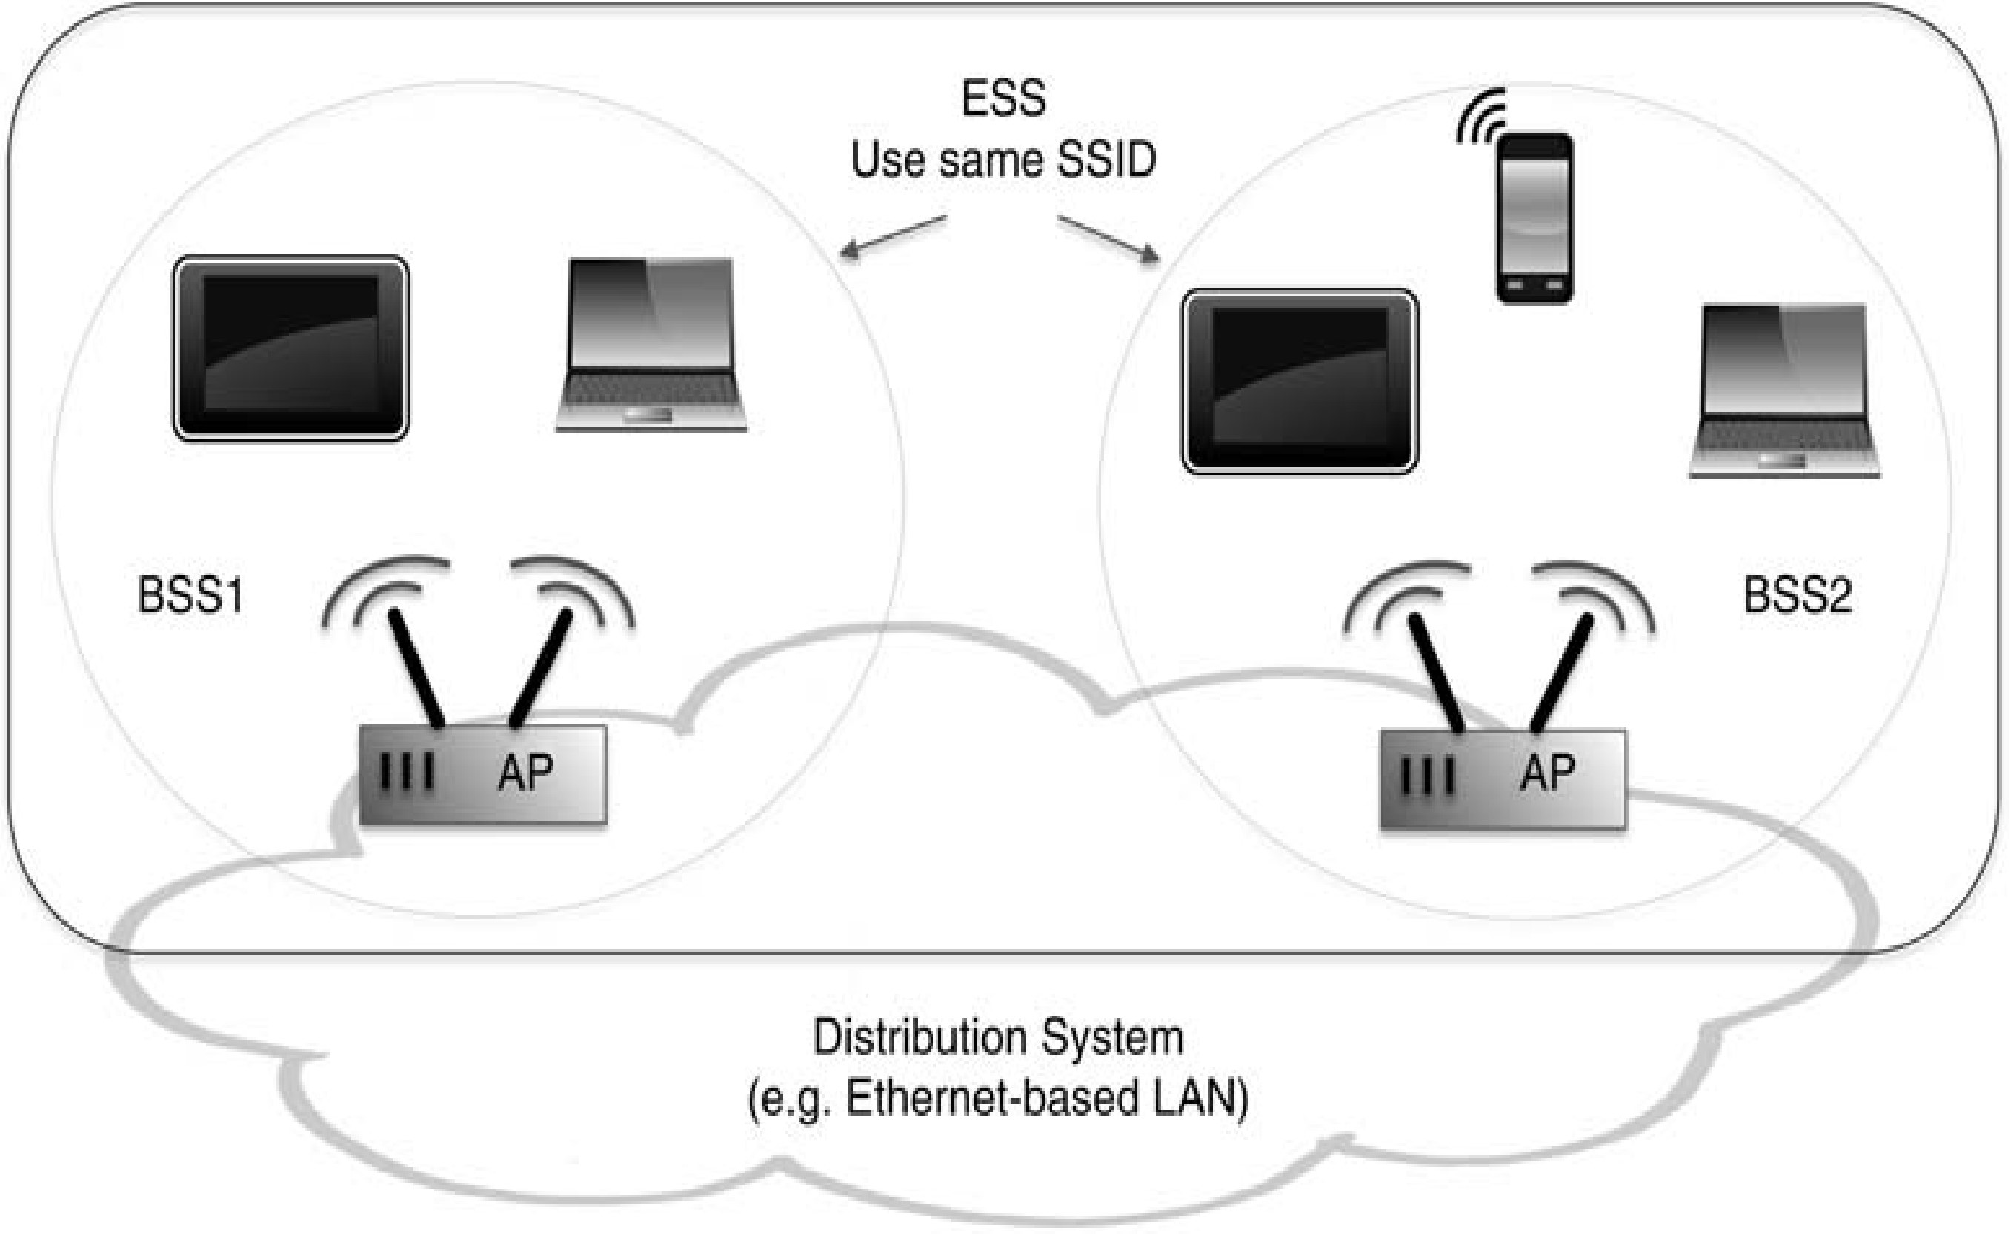
\includegraphics[scale=.27]{fig_tcc/arquiteturas_802-11_01.pdf}
		\caption*{{\footnotesize Fonte: Gorshe \textit{et al}. (2014, p. 308).}}
	\end{figure}
\end{frame}
% ----------------------------------------- Slide -----------------------------------------
\begin{frame}{Padrão IEEE 802.11}
	\begin{itemize}
		\item Resumo dos padrões IEEE 802.11.
	\end{itemize}
	\vspace*{-.5cm}
	\begin{figure}[H]
		\centering
		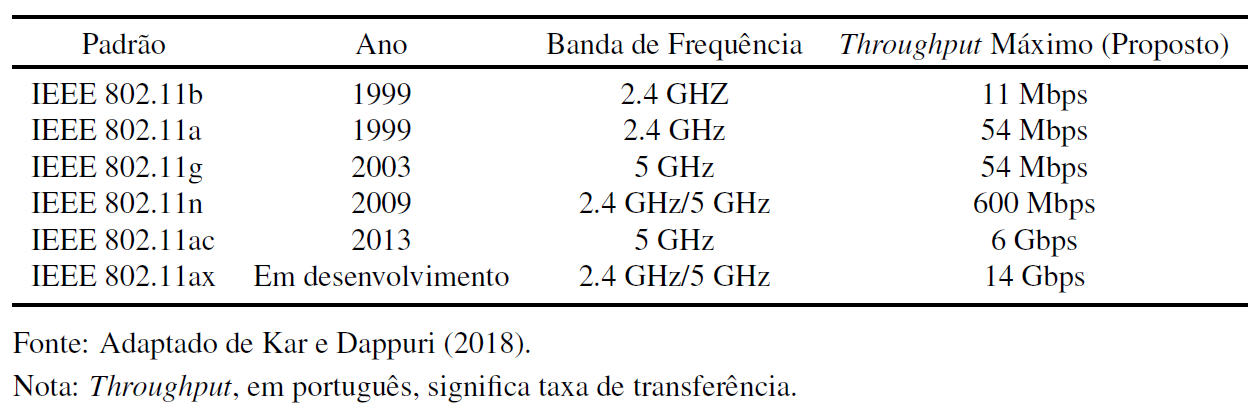
\includegraphics[scale=.445]{fig_tcc/ieee_802_11.png}
	\end{figure}
\end{frame}
% ----------------------------------------- Slide -----------------------------------------
\section{Site Survey}
% ----------------------------------------- Slide -----------------------------------------
\begin{frame}{Site Survey}
	\begin{figure}[H]
		\centering
		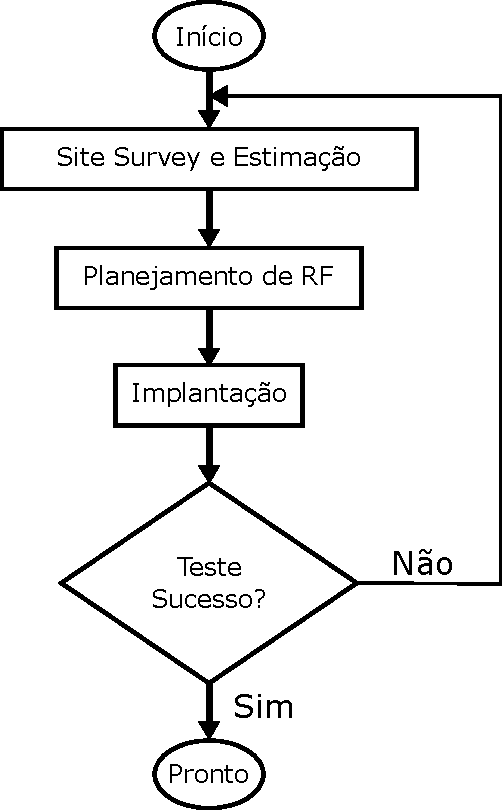
\includegraphics[scale=.45]{fig_tcc/fluxograma_site_survey_01.pdf}
		\caption*{{\footnotesize Fonte: Adaptado de Kar e Dappuri (2018).}}
	\end{figure}
\end{frame}
% ----------------------------------------- Slide -----------------------------------------
\section{Metodologia}
% ----------------------------------------- Slide -----------------------------------------
\begin{frame}{Metodologia}
	\vspace*{-.1cm}
	\begin{figure}[H]
		\centering
		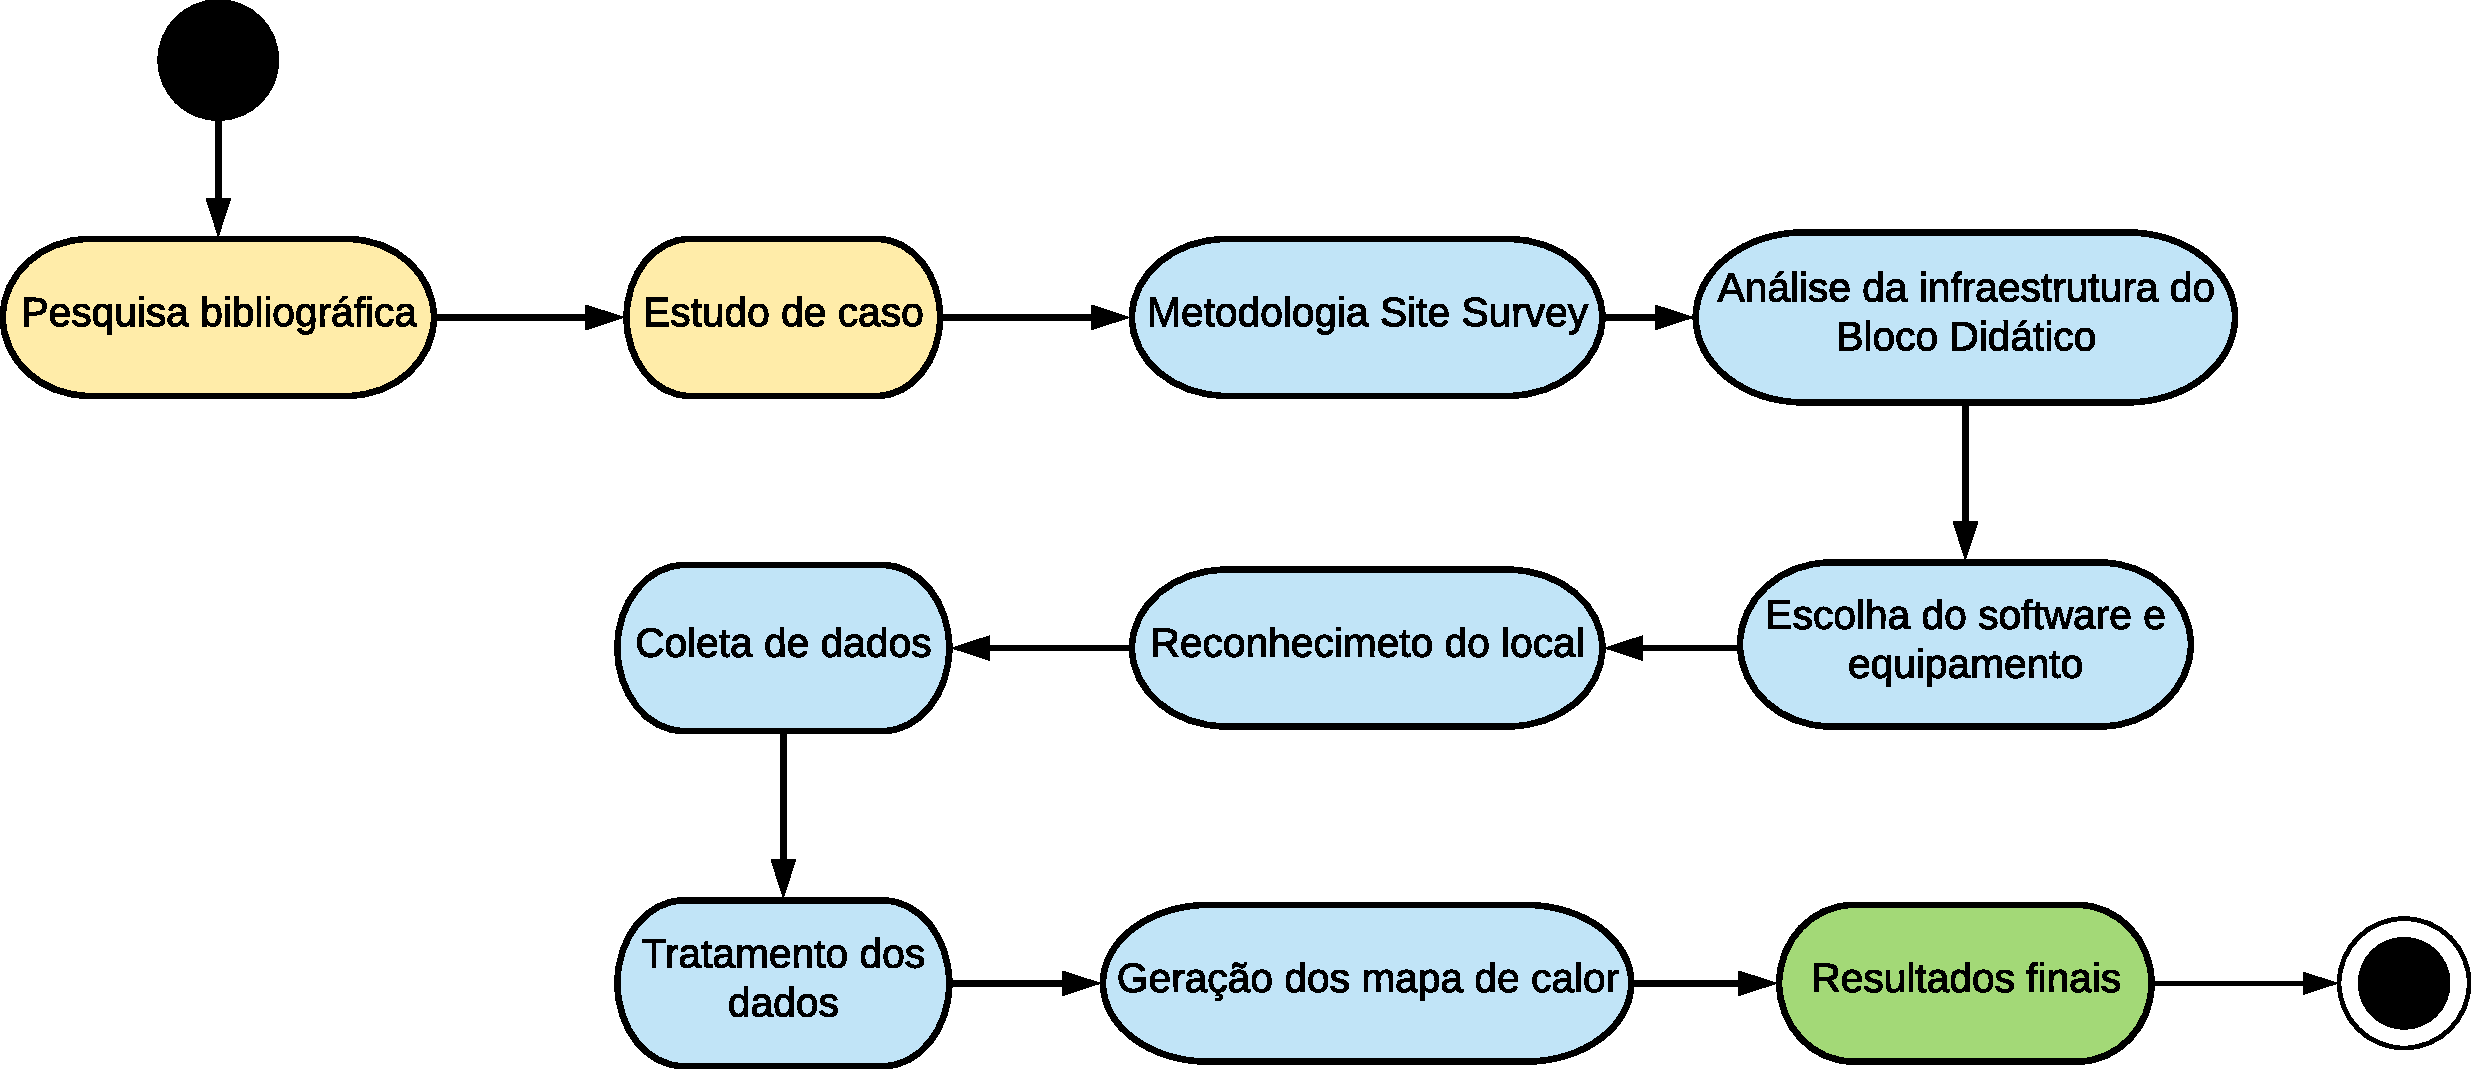
\includegraphics[scale=.32]{fig_tcc/slide_metodologia.pdf}
		\caption*{{\footnotesize Fonte: Autor.}}
	\end{figure}
\end{frame}
% ----------------------------------------- Slide -----------------------------------------
\begin{frame}{Softwares}
	\noindent
	\begin{minipage}[c]{0.48\linewidth}
		\begin{figure}[H]
			\caption*{{\fontsize{9pt}{11}\selectfont Ekahau Heatmapper.}}
			\centering
			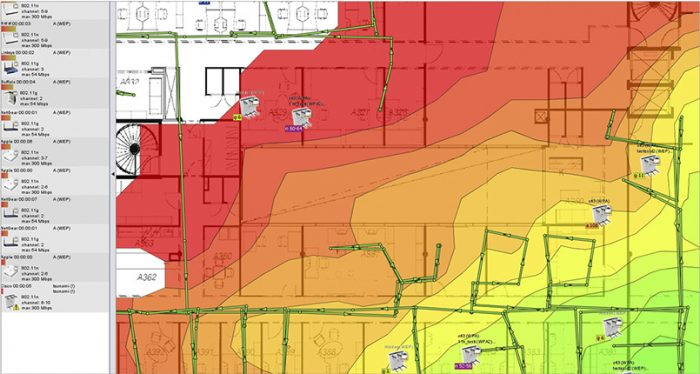
\includegraphics[scale=.29]{fig_tcc/heatmapper.jpg}
			\caption*{{\fontsize{9pt}{11}\selectfont Ekahau\ldots (c2019).}}
		\end{figure}
	\end{minipage}
	\hfill%
	\begin{minipage}[c]{.48\linewidth}
		\begin{figure}[H]
			\centering
			\caption*{{\fontsize{9pt}{11}\selectfont Xirrus Wi-Fi Inspector.}}
			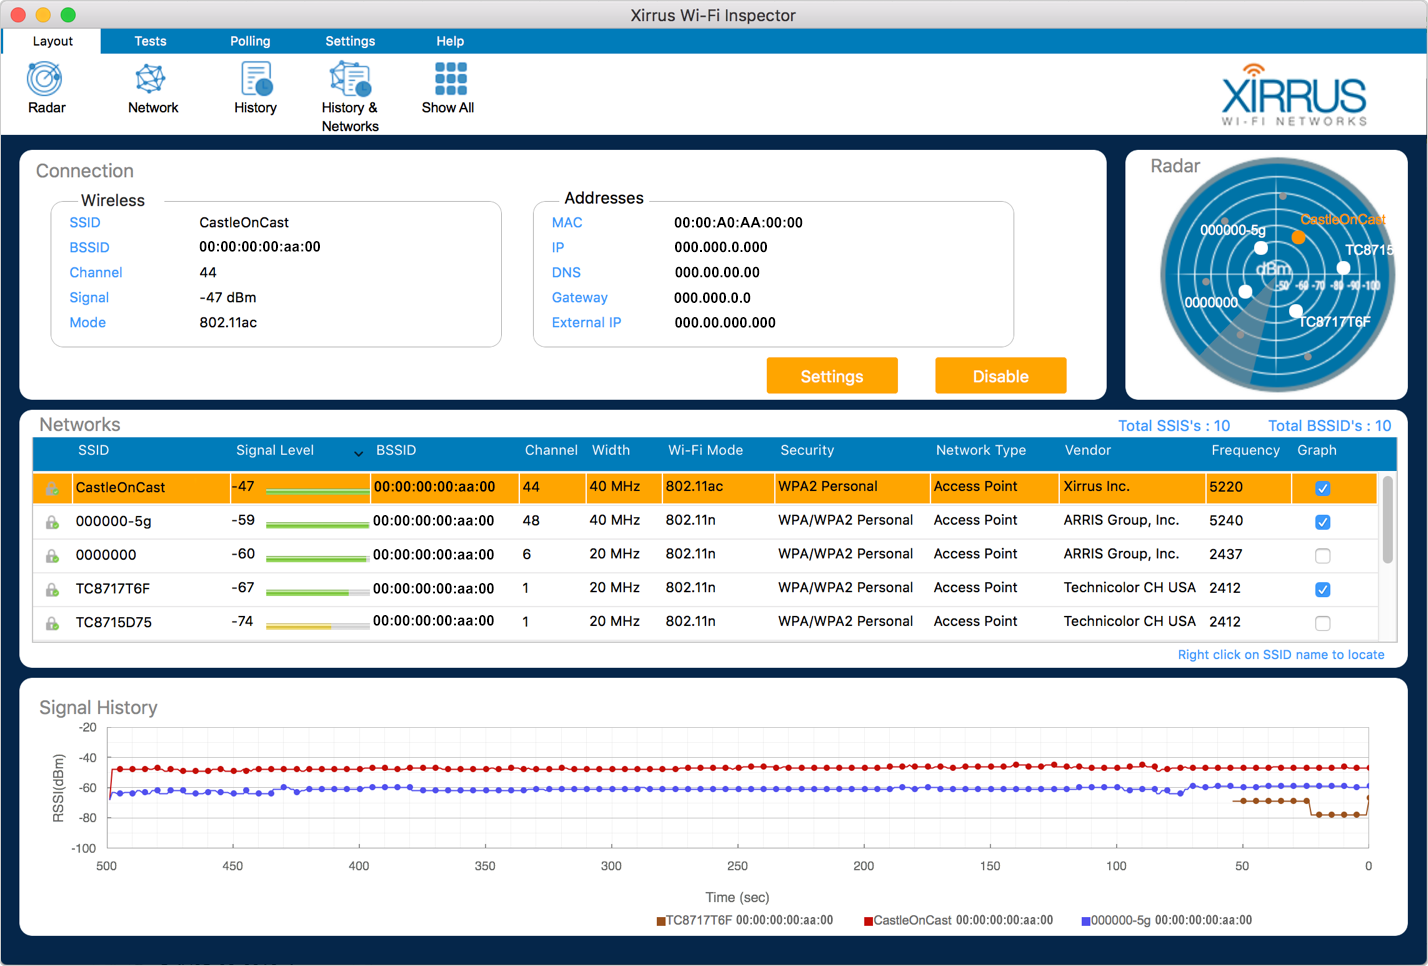
\includegraphics[scale=0.133]{fig_tcc/xirrus.png}
			\caption*{{\fontsize{9pt}{11}\selectfont Fonte: Wi-Fi\ldots (c2019).}}
		\end{figure}
	\end{minipage}
\end{frame}
% ----------------------------------------- Slide -----------------------------------------
\section{Materiais Utilizados}
% ----------------------------------------- Slide -----------------------------------------
\begin{frame}{Hardware}
	\noindent
	\begin{minipage}[c]{0.48\linewidth}
		\begin{figure}[H]
			\centering
			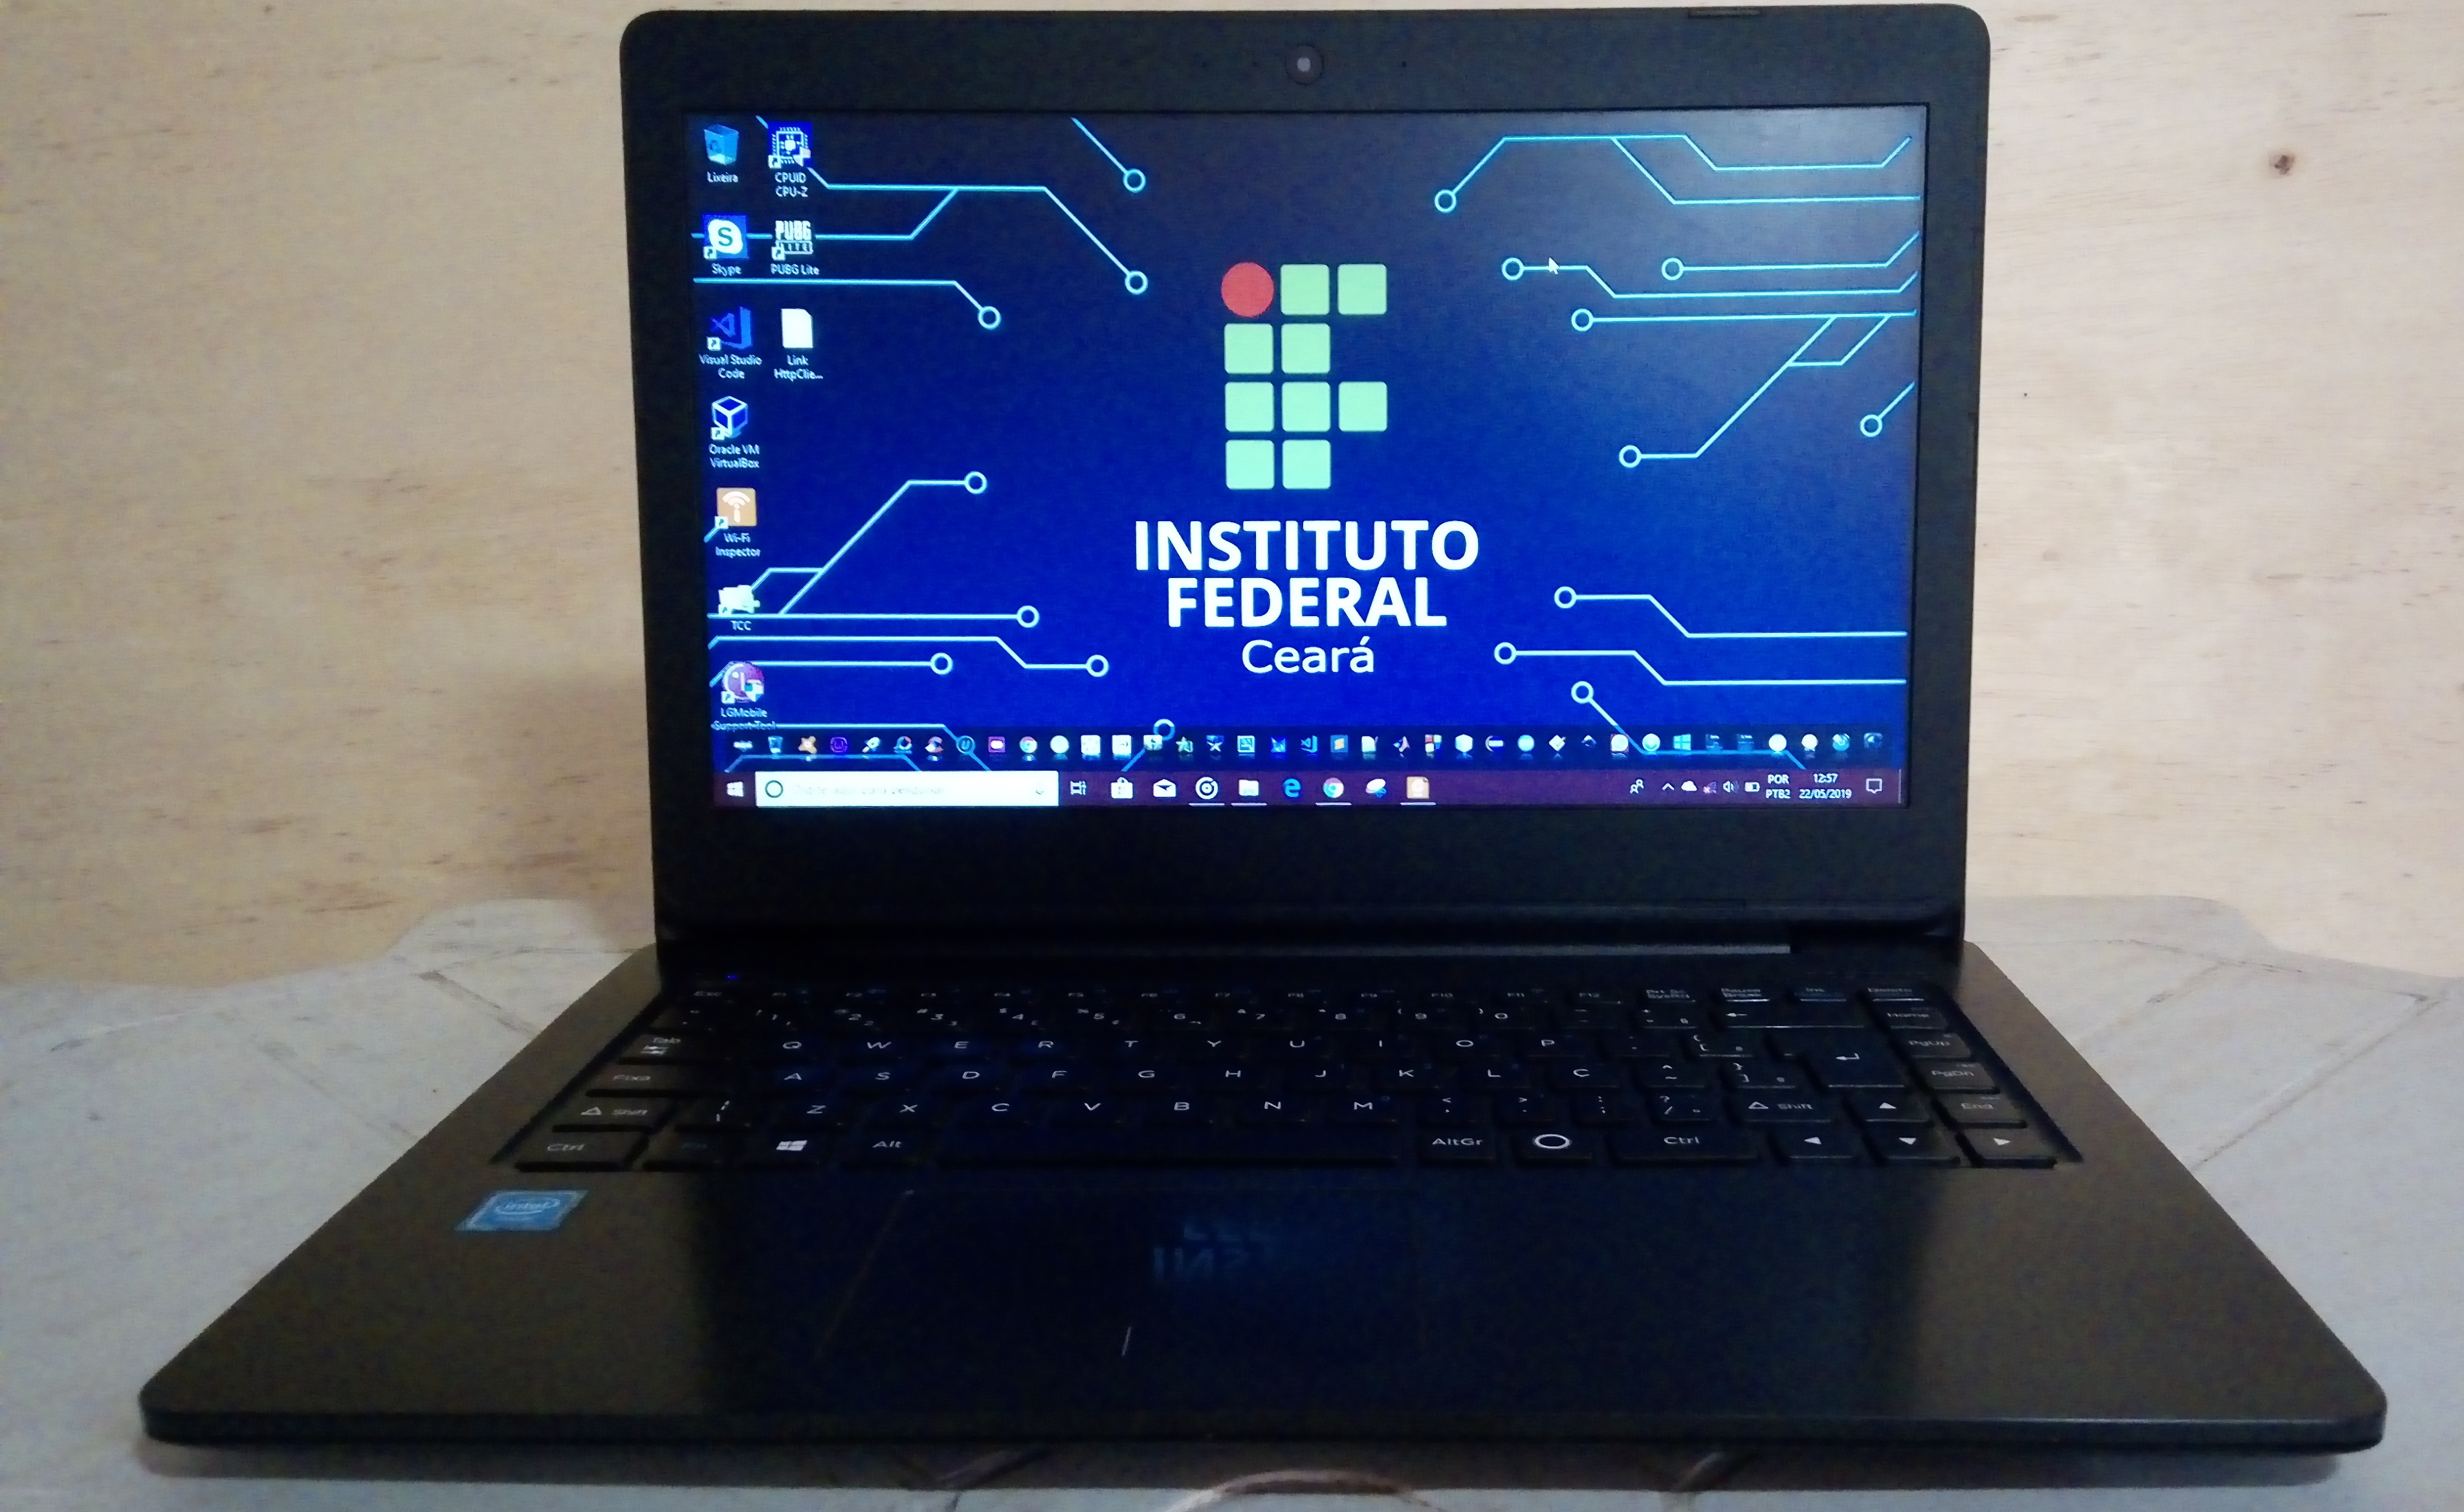
\includegraphics[scale=.0535]{fig_tcc/notebook.jpg}
			\caption*{{\footnotesize Fonte: Autor.}}
		\end{figure}
	\end{minipage}
	\hfill%
	\begin{minipage}[c]{.48\linewidth}
		\begin{figure}[H]
			\centering
			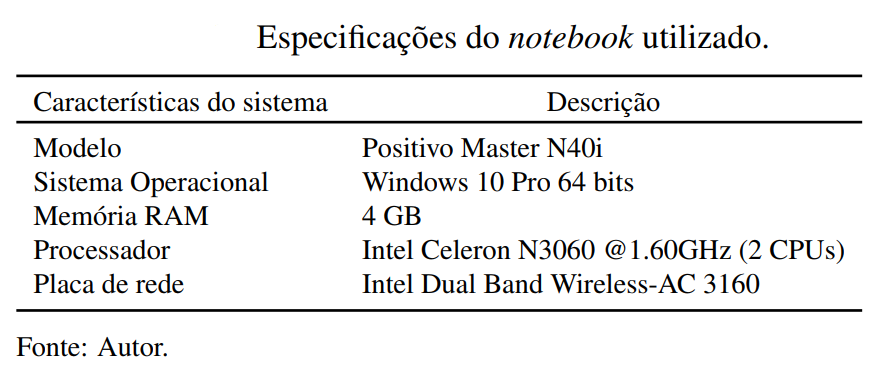
\includegraphics[scale=0.3]{fig_tcc/tab_notebook.png}
		\end{figure}
	\end{minipage}
\end{frame}
% ----------------------------------------- Slide -----------------------------------------
\section{Resultados}
% ----------------------------------------- Slide -----------------------------------------
\begin{frame}{Primeiro Andar do Bloco Didático}
	\vspace*{-3mm}
		\begin{figure}[H]
		\centering
		\caption*{{\fontsize{9pt}{11}\selectfont Planta Baixa do 1º andar.}}
		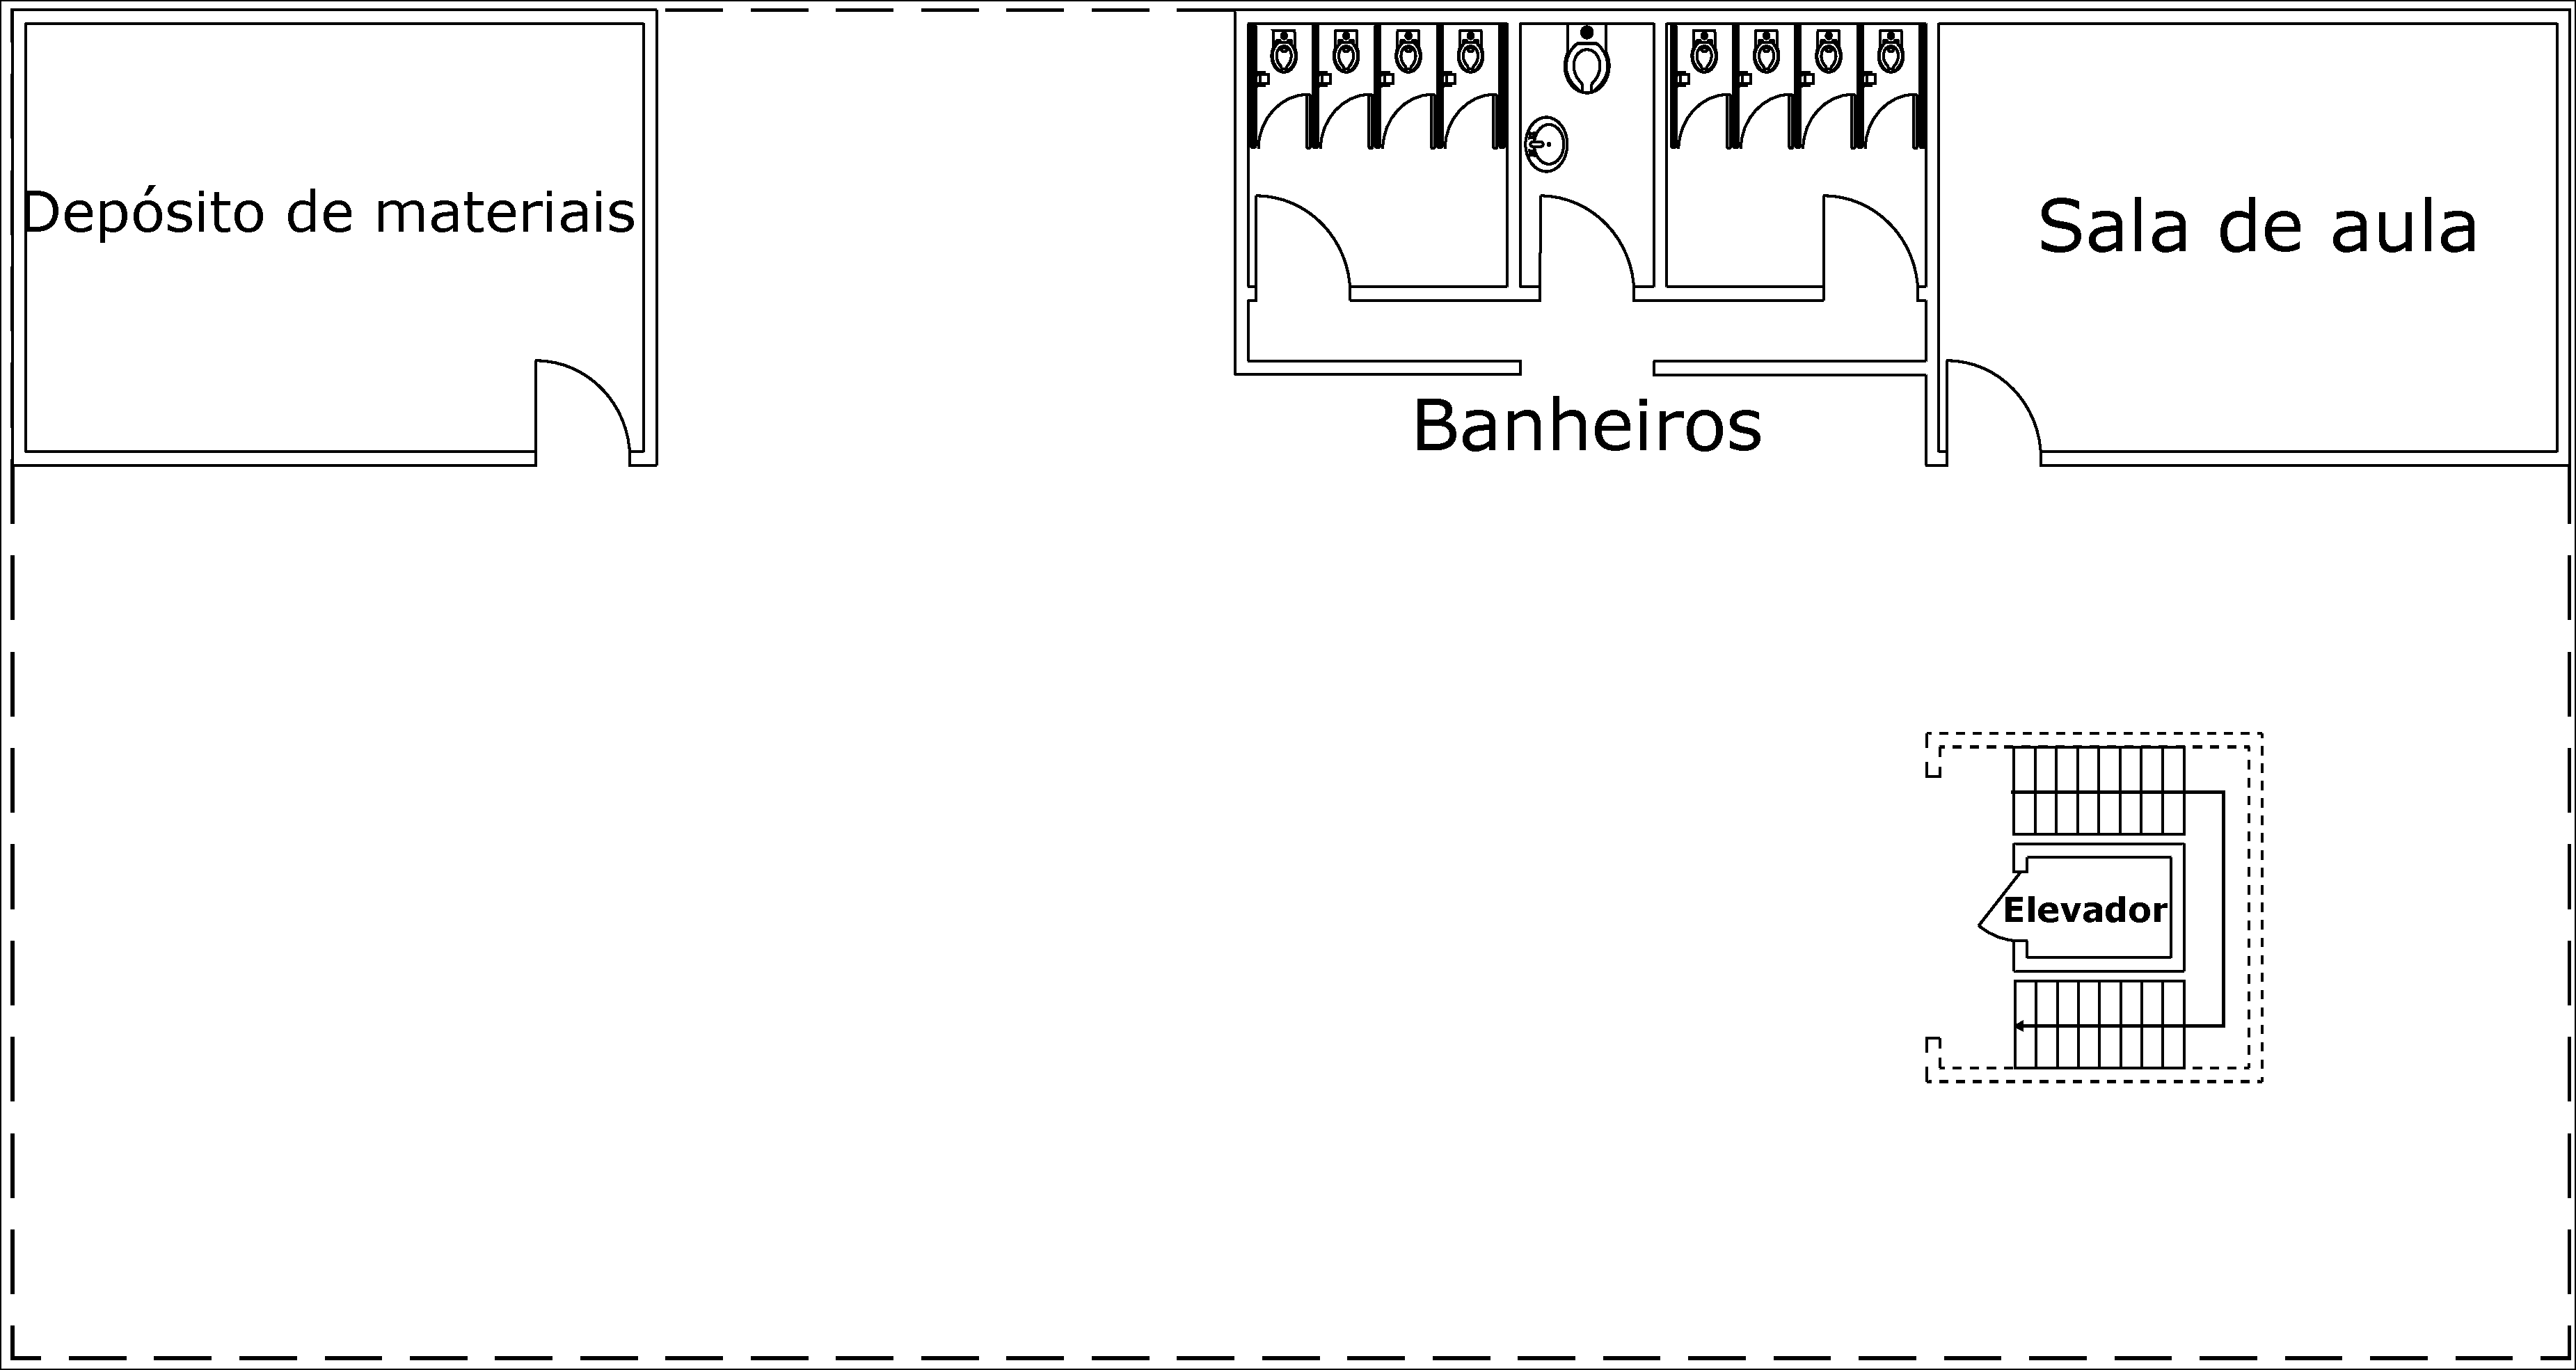
\includegraphics[scale=0.16]{fig_tcc/planta_andar1.pdf}
		\caption*{{\fontsize{9pt}{11}\selectfont Fonte: Autor.}}
	\end{figure}
\end{frame}
% ----------------------------------------- Slide -----------------------------------------
\begin{frame}{Primeiro Andar do Bloco Didático}
	\framesubtitle{Pontos Medidos}
	\vspace*{-3mm}
	\begin{figure}[H]
		\centering
		\caption*{{\fontsize{9pt}{11}\selectfont Pontos medidos no 1º andar.}}
		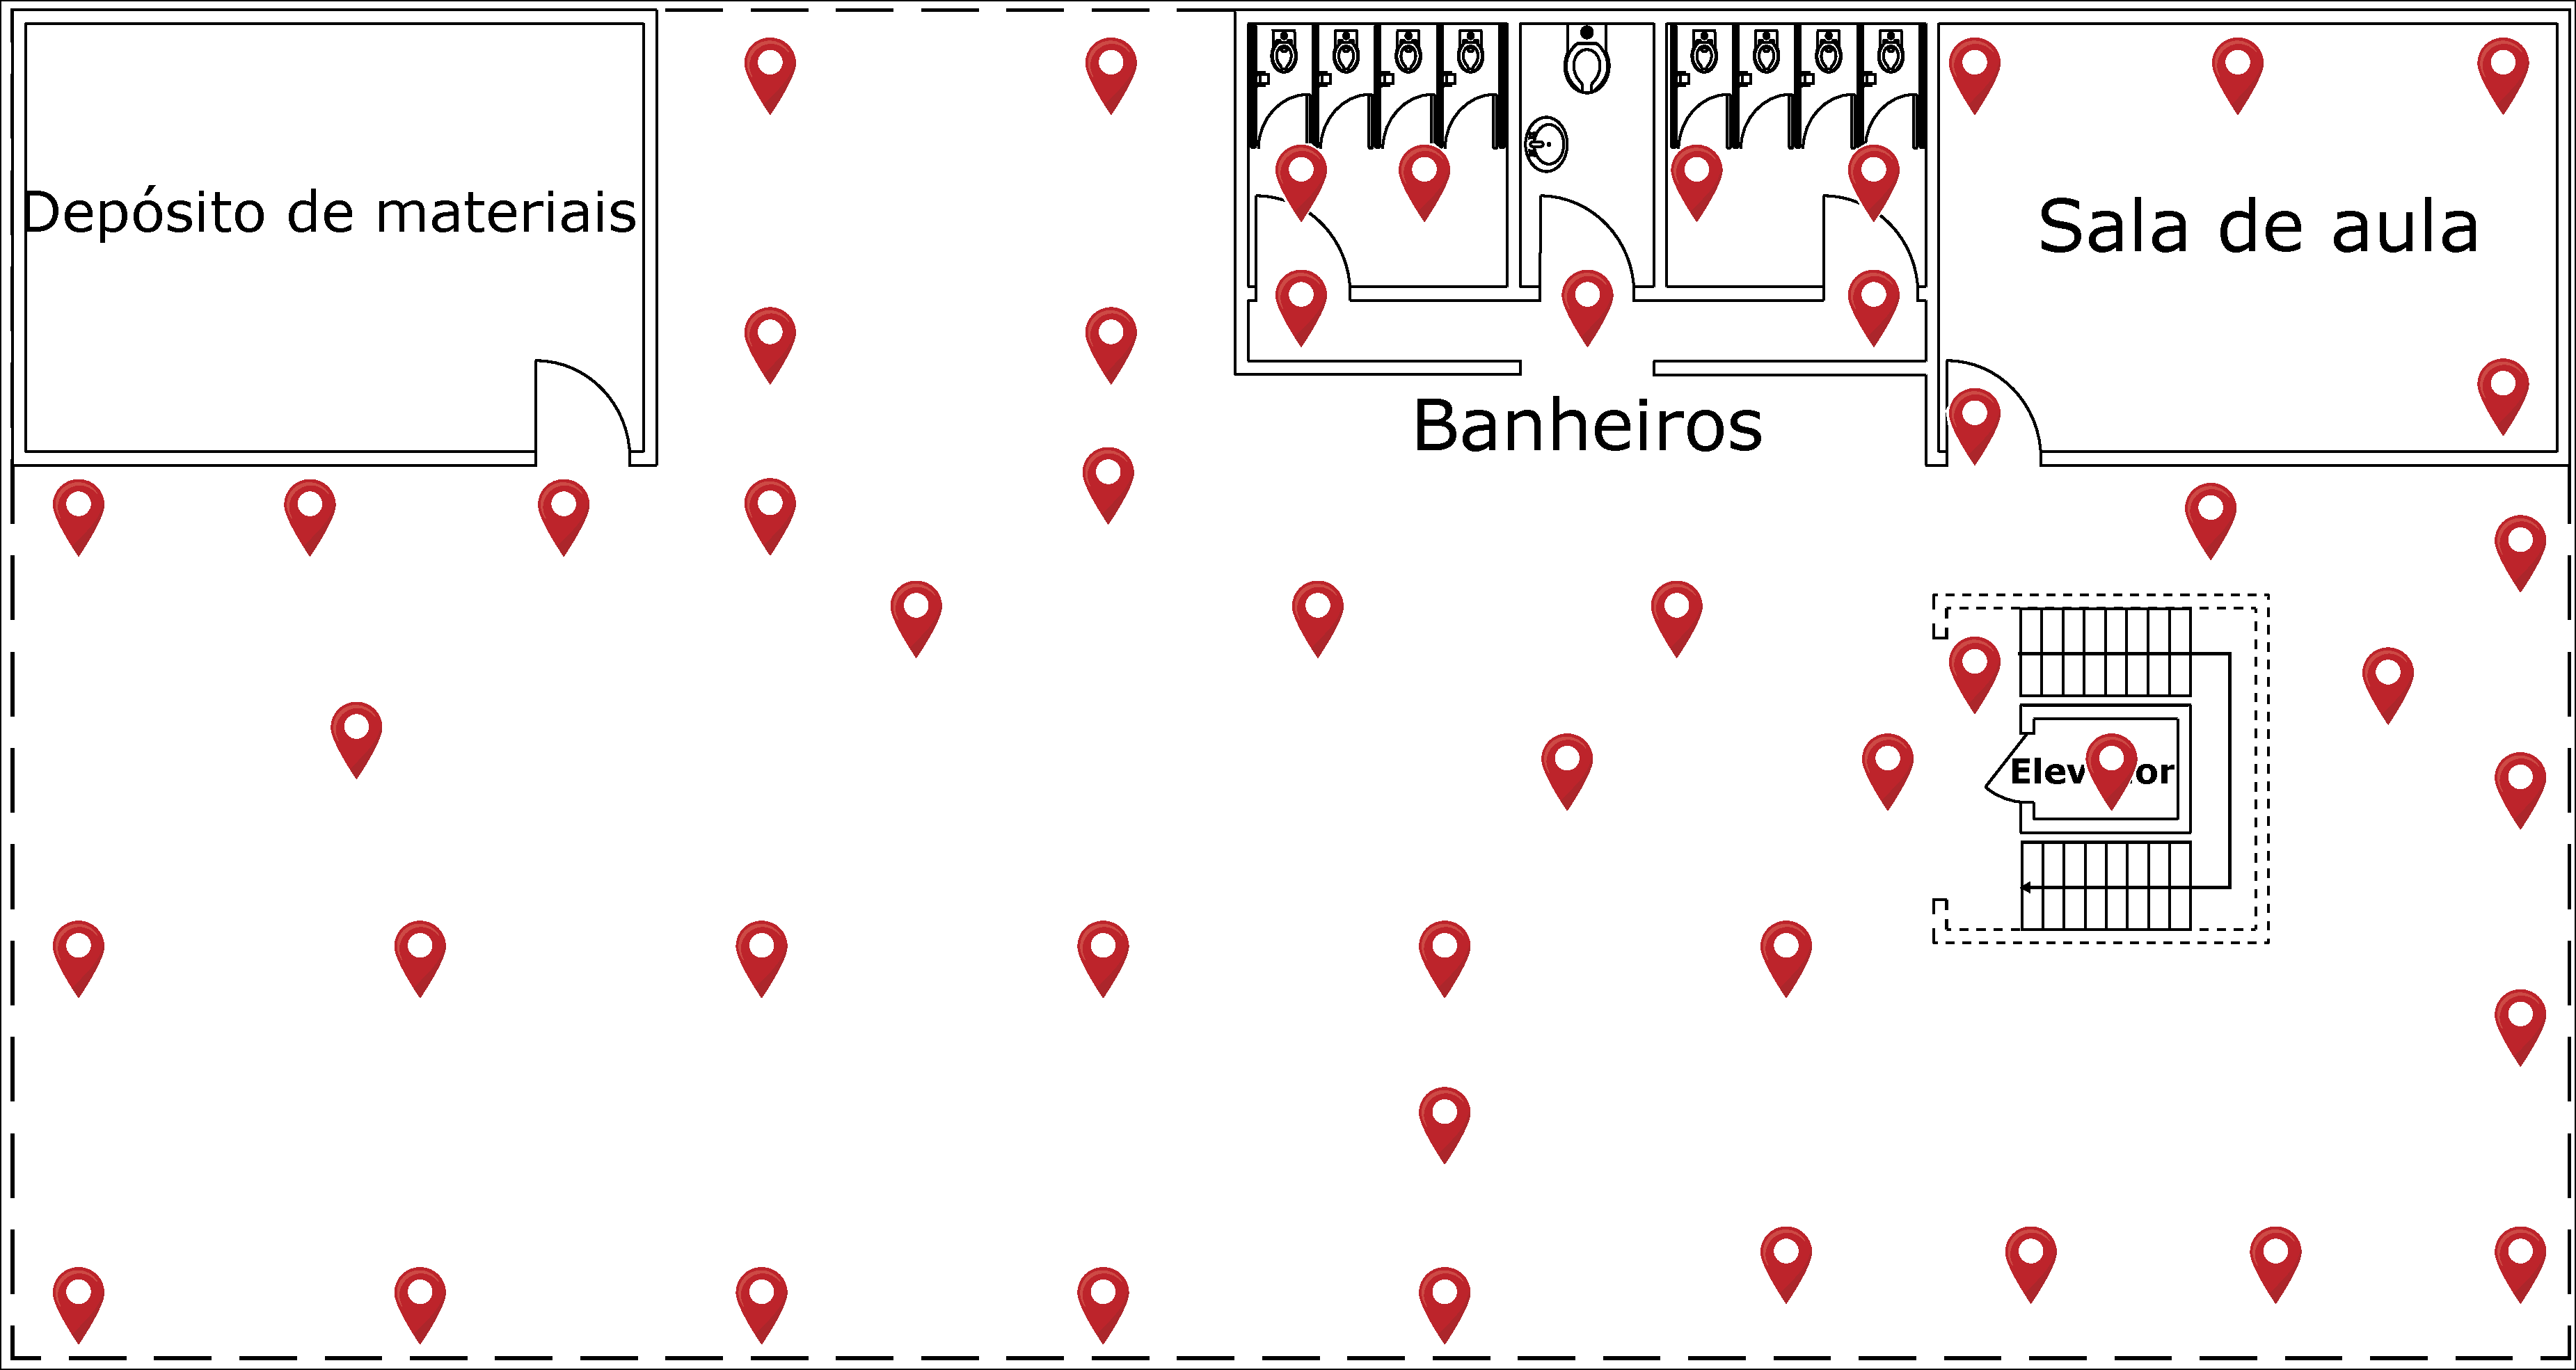
\includegraphics[scale=0.14]{fig_tcc/Pontos_Medidos_Andar01.pdf}
		\caption*{{\fontsize{9pt}{11}\selectfont Fonte: Autor.}}
	\end{figure}
\end{frame}
% ----------------------------------------- Slide -----------------------------------------
\begin{frame}{Primeiro Andar do Bloco Didático}
	\framesubtitle{Mapa de Calor}
	\vspace*{-3mm}
	\begin{figure}[H]
		\centering
		\caption*{{\fontsize{9pt}{11}\selectfont Mapa de calor do 1º andar.}}
		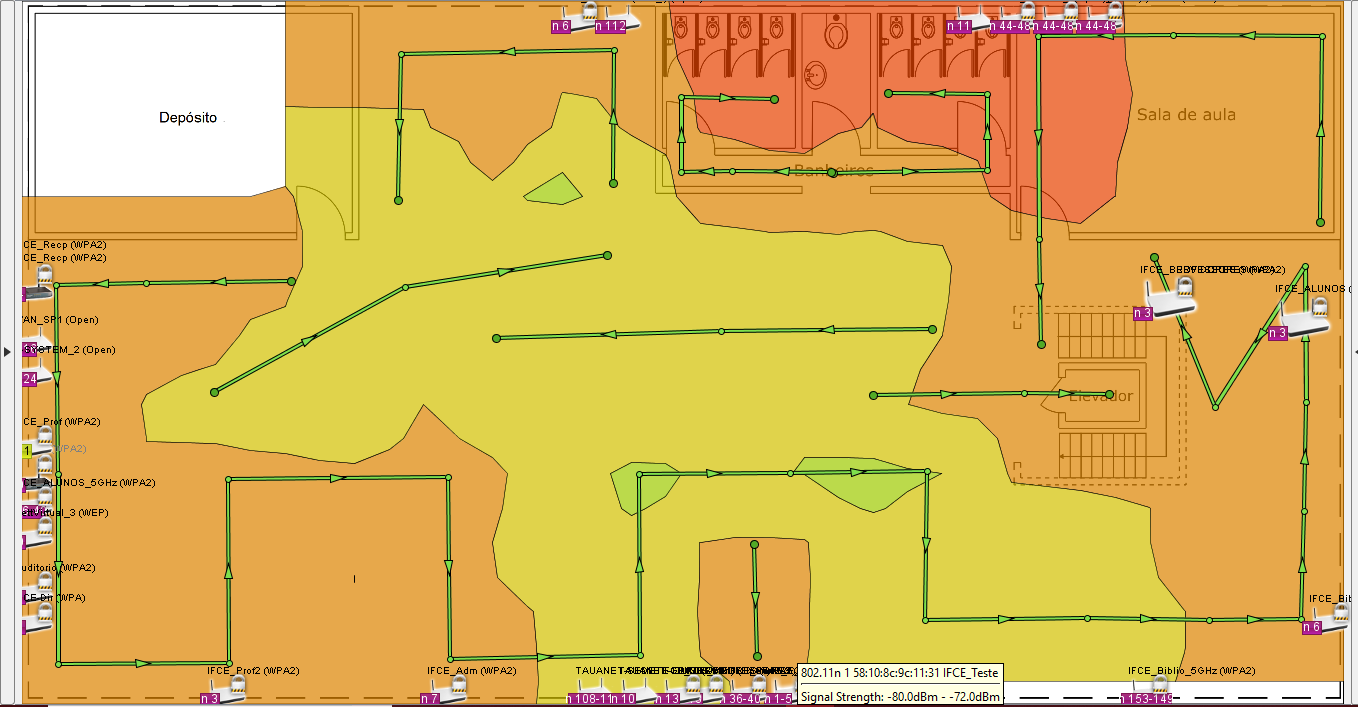
\includegraphics[scale=0.28]{fig_tcc/heatmapper_Terreo_Editada.png}
		\caption*{{\fontsize{8pt}{11}\selectfont Fonte: Autor.}}
	\end{figure}
\end{frame}
% ----------------------------------------- Slide -----------------------------------------
% Segundo Andar
\begin{frame}{Segundo Andar do Bloco Didático}
	\vspace*{-3mm}
	\begin{figure}[H]
		\centering
		\caption*{{\fontsize{9pt}{11}\selectfont Planta Baixa do 2º andar.}}
		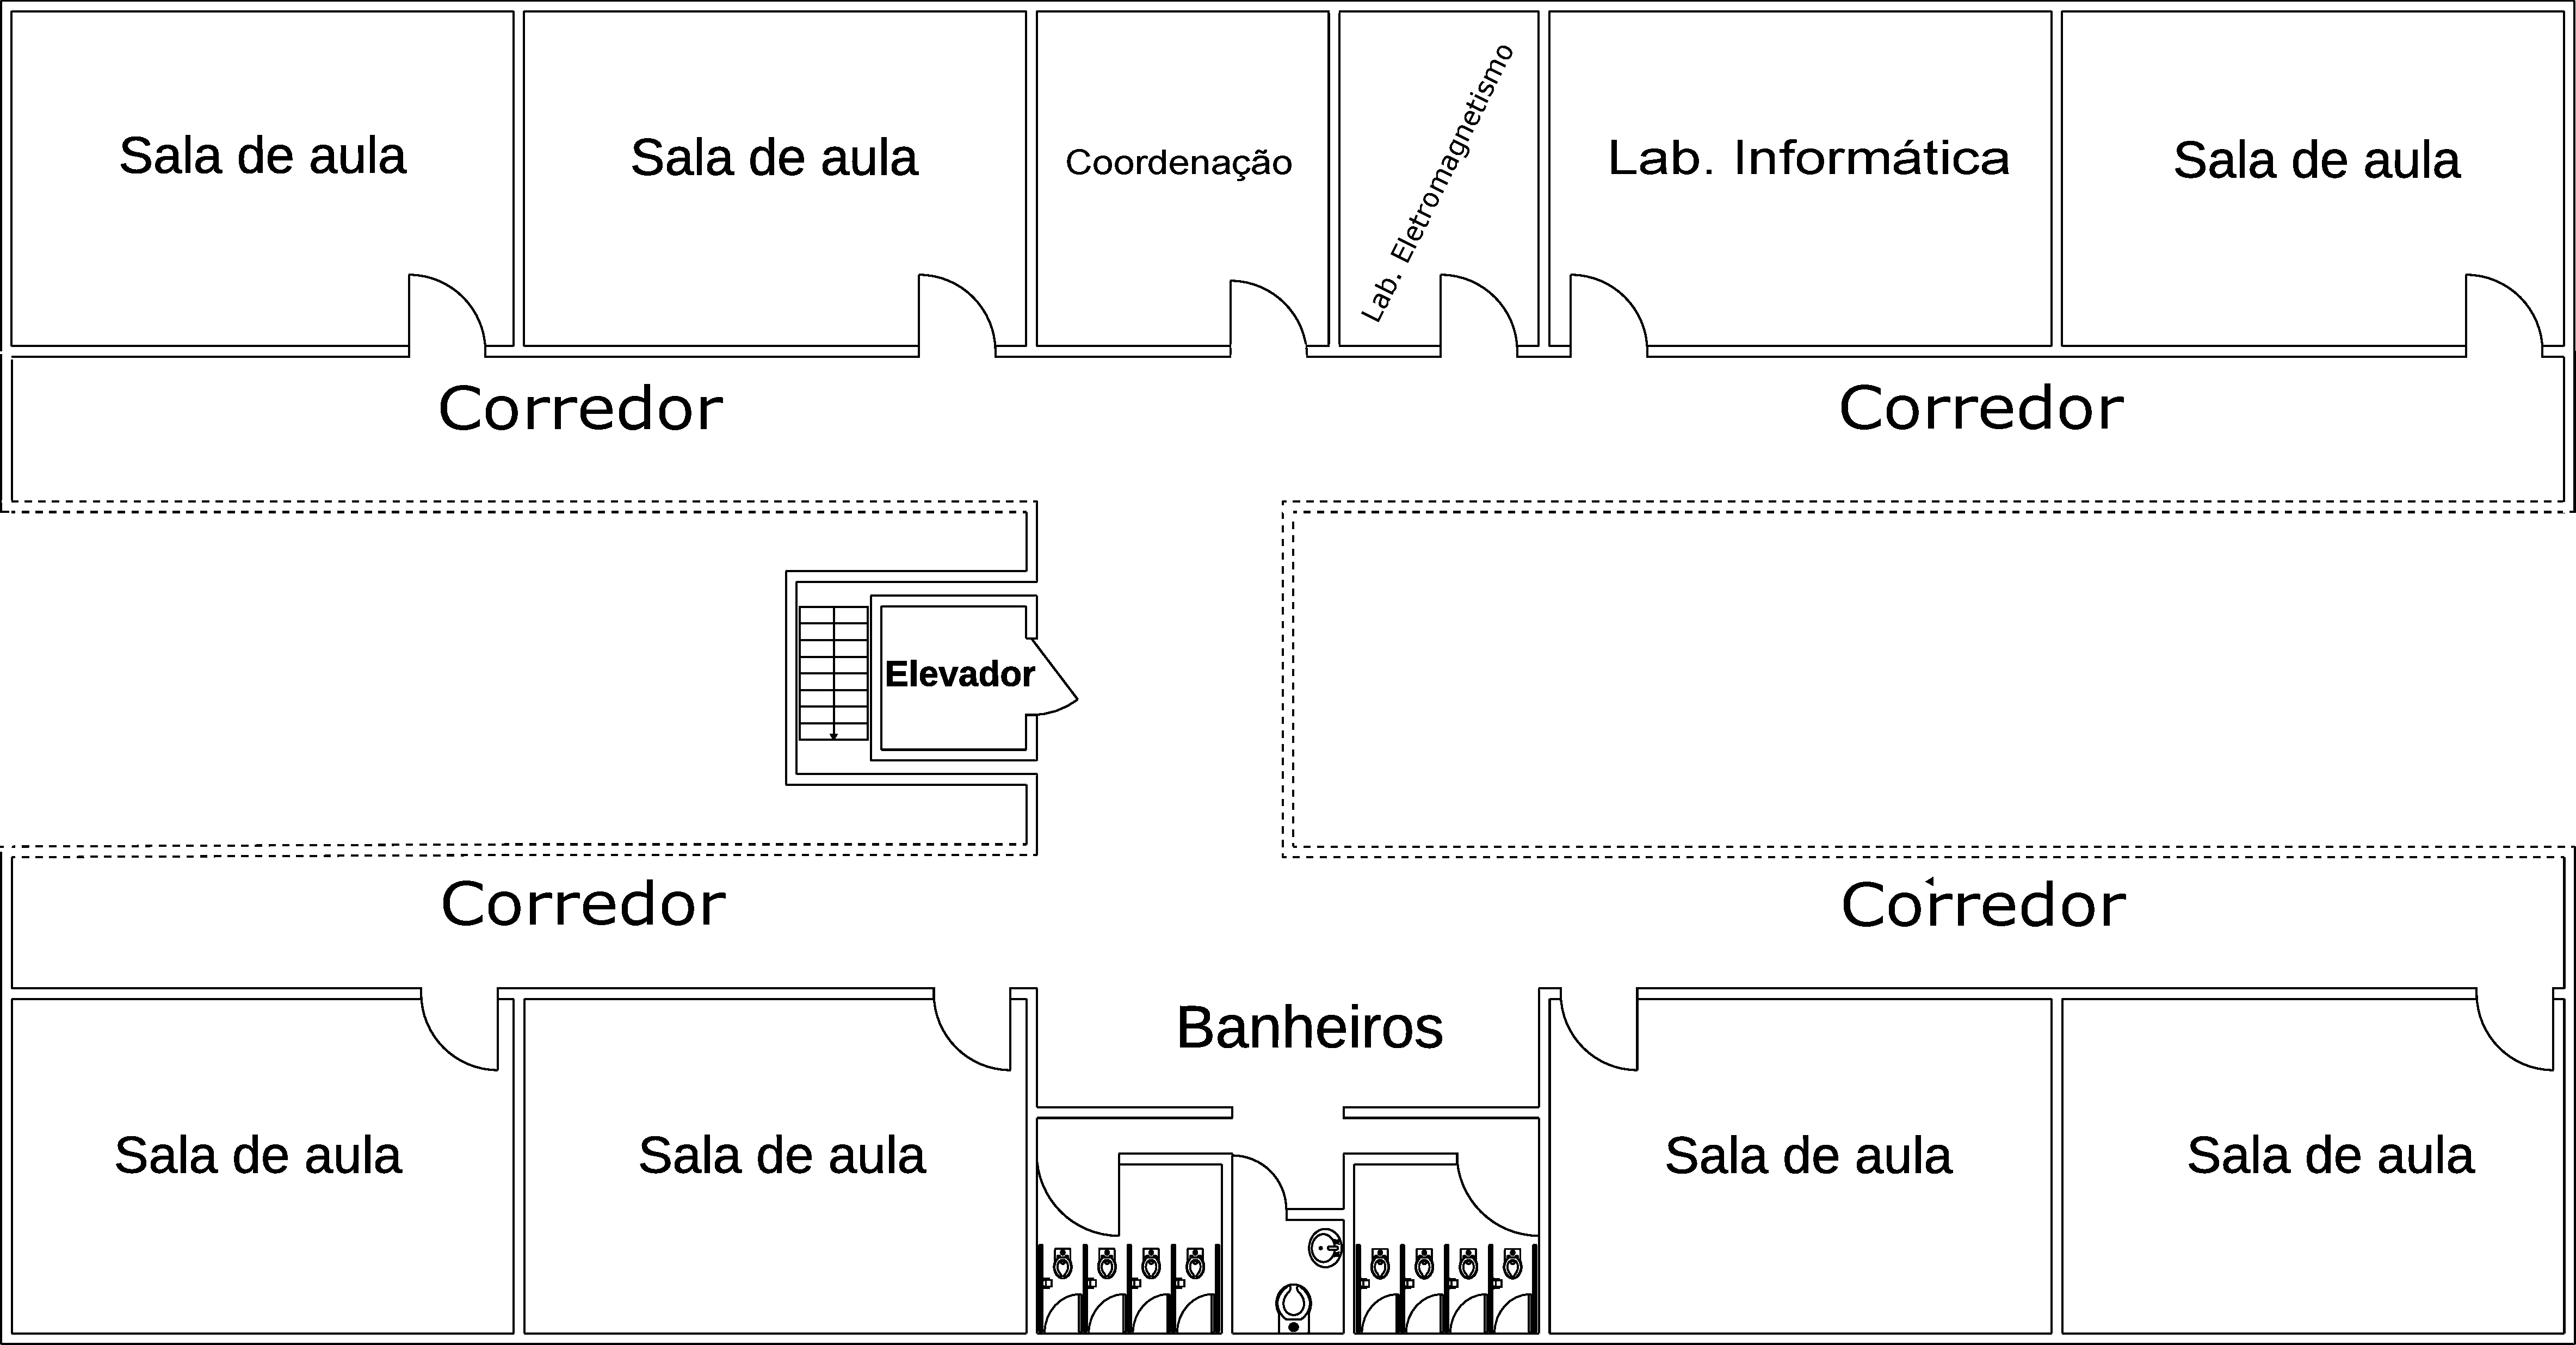
\includegraphics[scale=0.135]{fig_tcc/planta_andar2.pdf}
		\caption*{{\fontsize{9pt}{11}\selectfont Fonte: Autor.}}
	\end{figure}
\end{frame}
% ----------------------------------------- Slide -----------------------------------------
\begin{frame}{Segundo Andar do Bloco Didático}
	\framesubtitle{Pontos Medidos}
	\vspace*{-3mm}
	\begin{figure}[H]
		\centering
		\caption*{{\fontsize{9pt}{11}\selectfont Pontos medidos no 2º andar.}}
		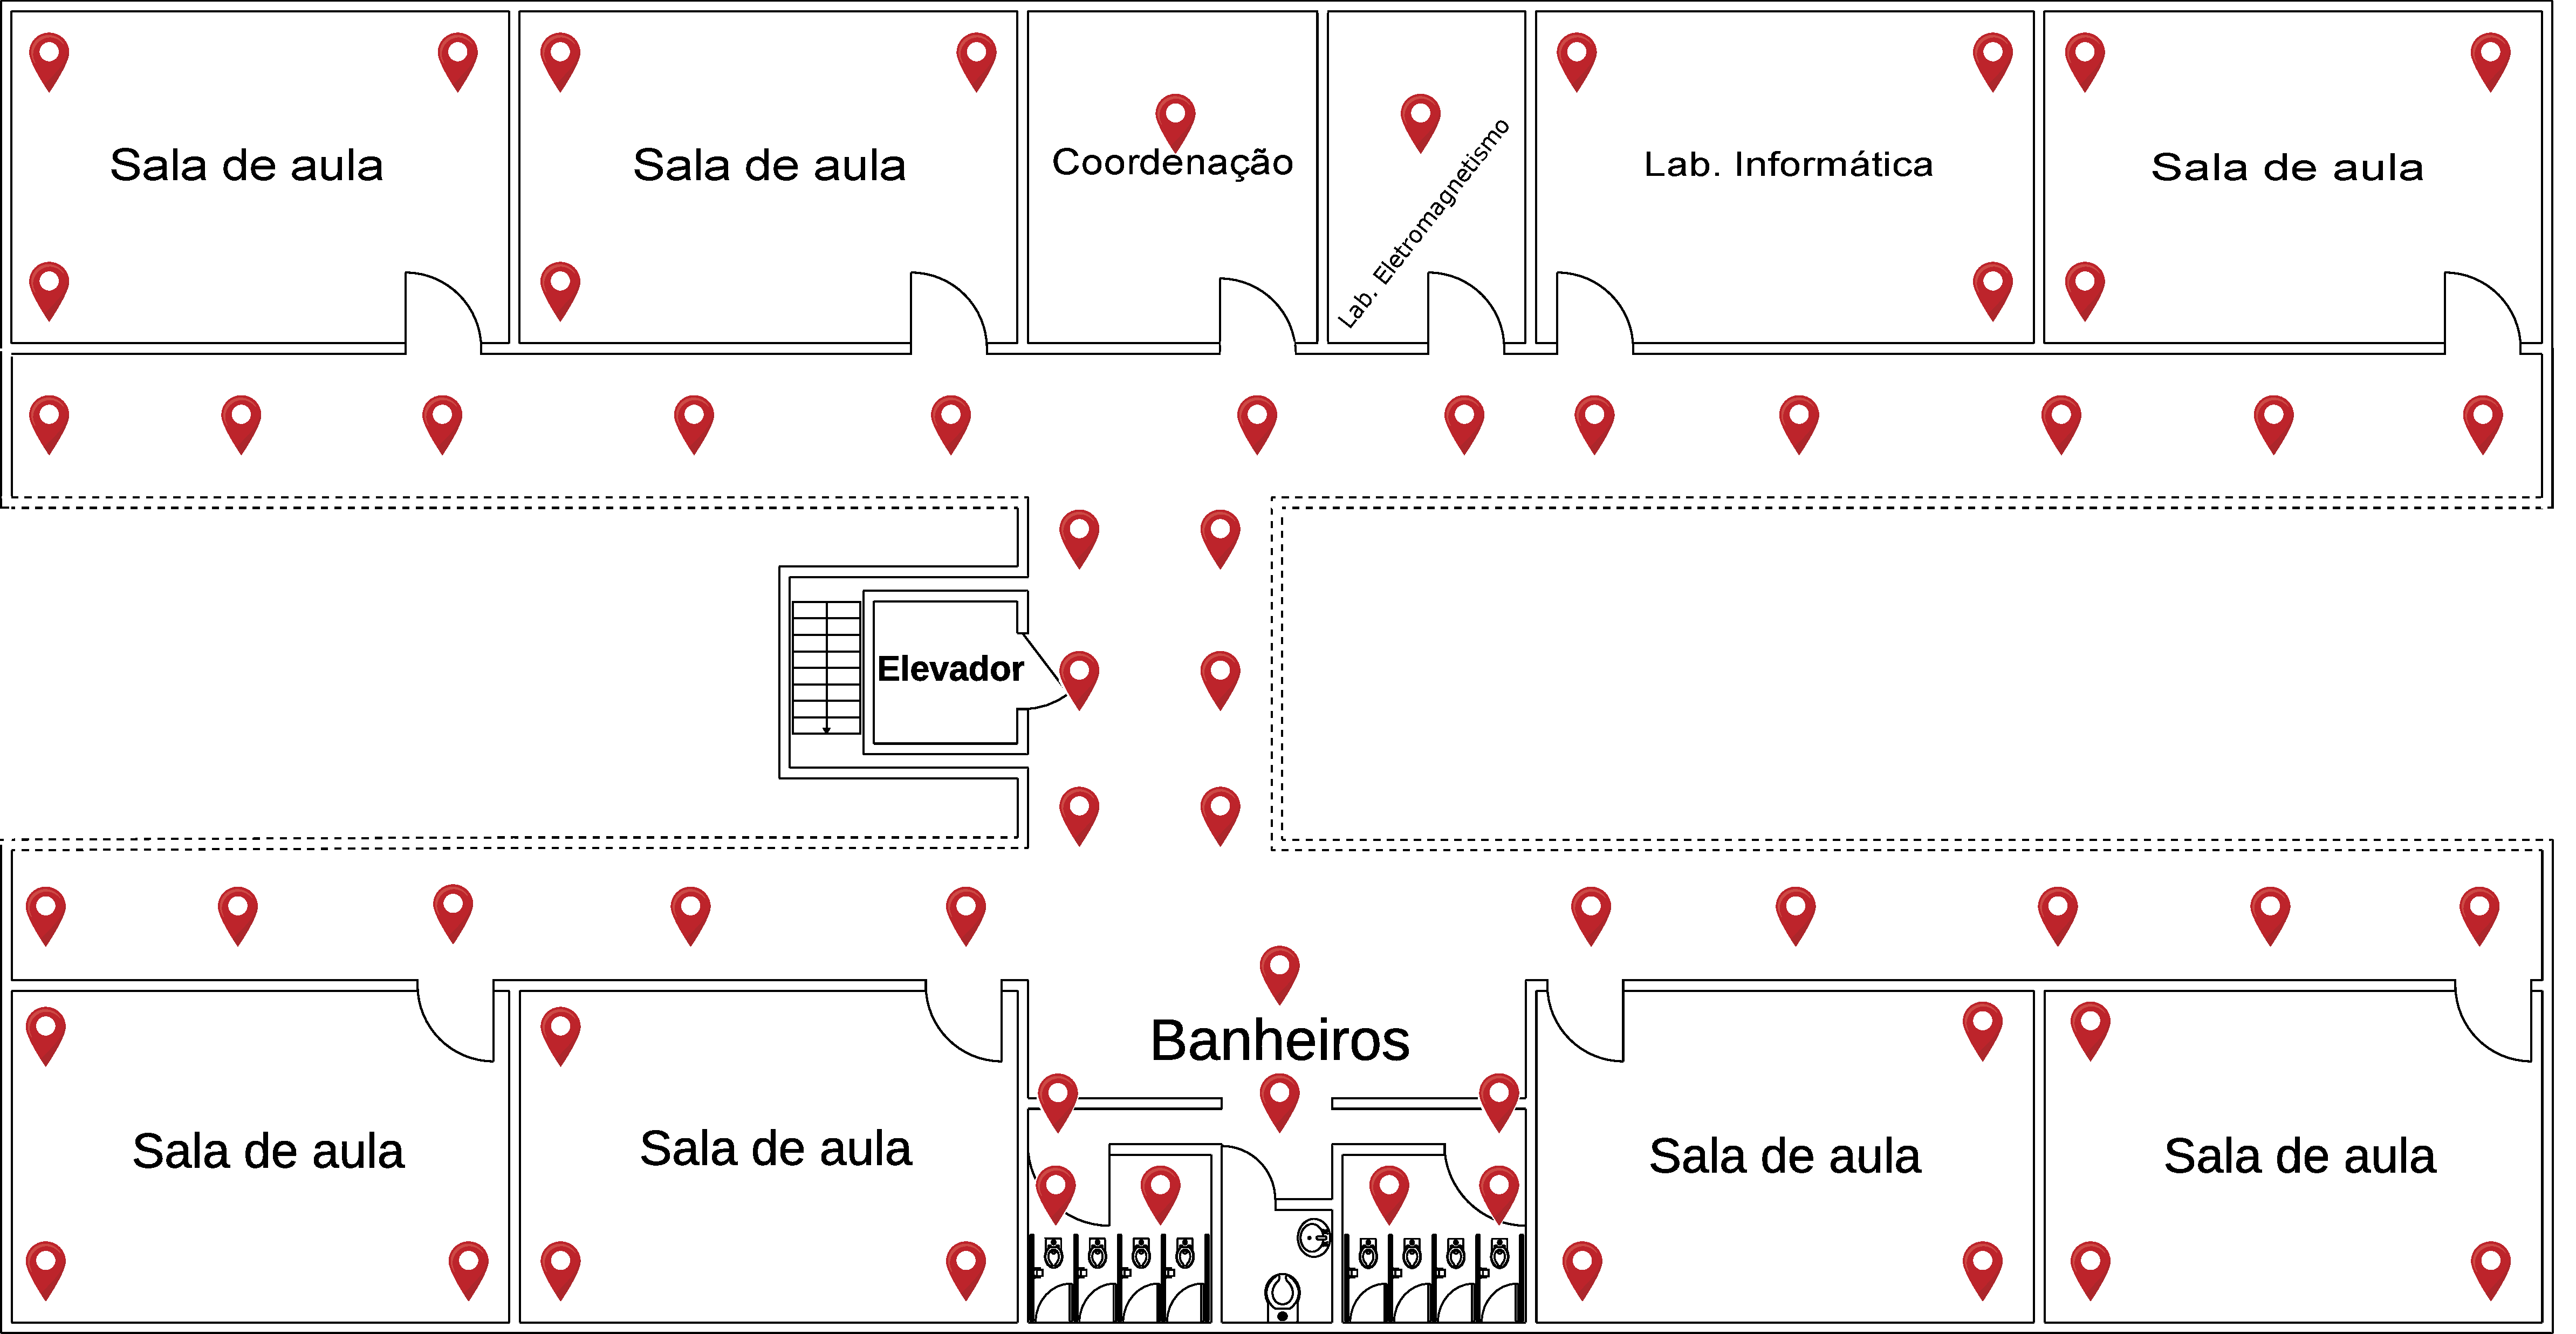
\includegraphics[scale=0.12]{fig_tcc/Pontos_Medidos_Andar02.pdf}
		\caption*{{\fontsize{9pt}{11}\selectfont Fonte: Autor.}}
	\end{figure}
\end{frame}
% ----------------------------------------- Slide -----------------------------------------
\begin{frame}{Segundo Andar do Bloco Didático}
	\framesubtitle{Mapa de Calor}
	\vspace*{-3mm}
	\begin{figure}[H]
		\centering
		\caption*{{\fontsize{9pt}{11}\selectfont Mapa de calor do 2º andar.}}
		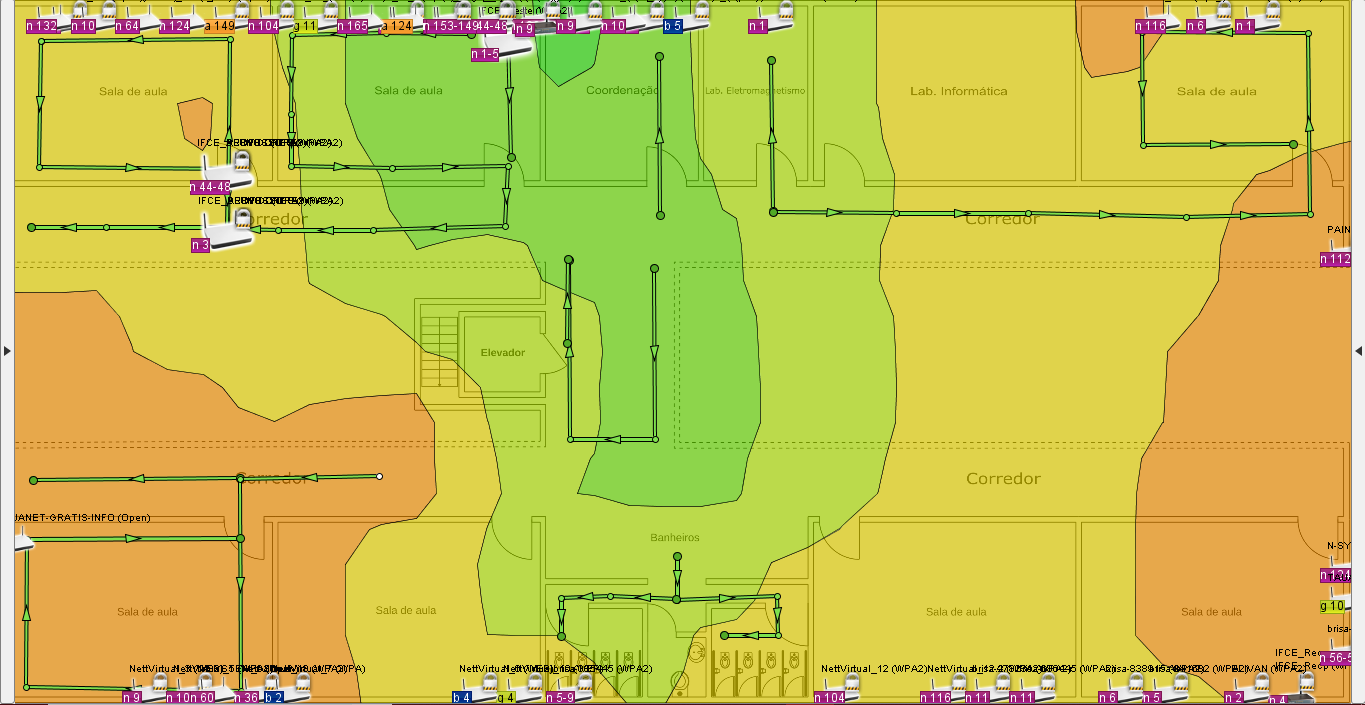
\includegraphics[scale=0.28]{fig_tcc/heatmapper_2_andar.png}
		\caption*{{\fontsize{8pt}{11}\selectfont Fonte: Autor.}}
	\end{figure}
\end{frame}
% ----------------------------------------- Slide -----------------------------------------
\section{Propostas de Intervenção}
% ----------------------------------------- Slide -----------------------------------------
\begin{frame}{Proposta para Melhoria do Sinal}
	\framesubtitle{Primeiro Andar}
	\begin{figure}[H]
		\centering
		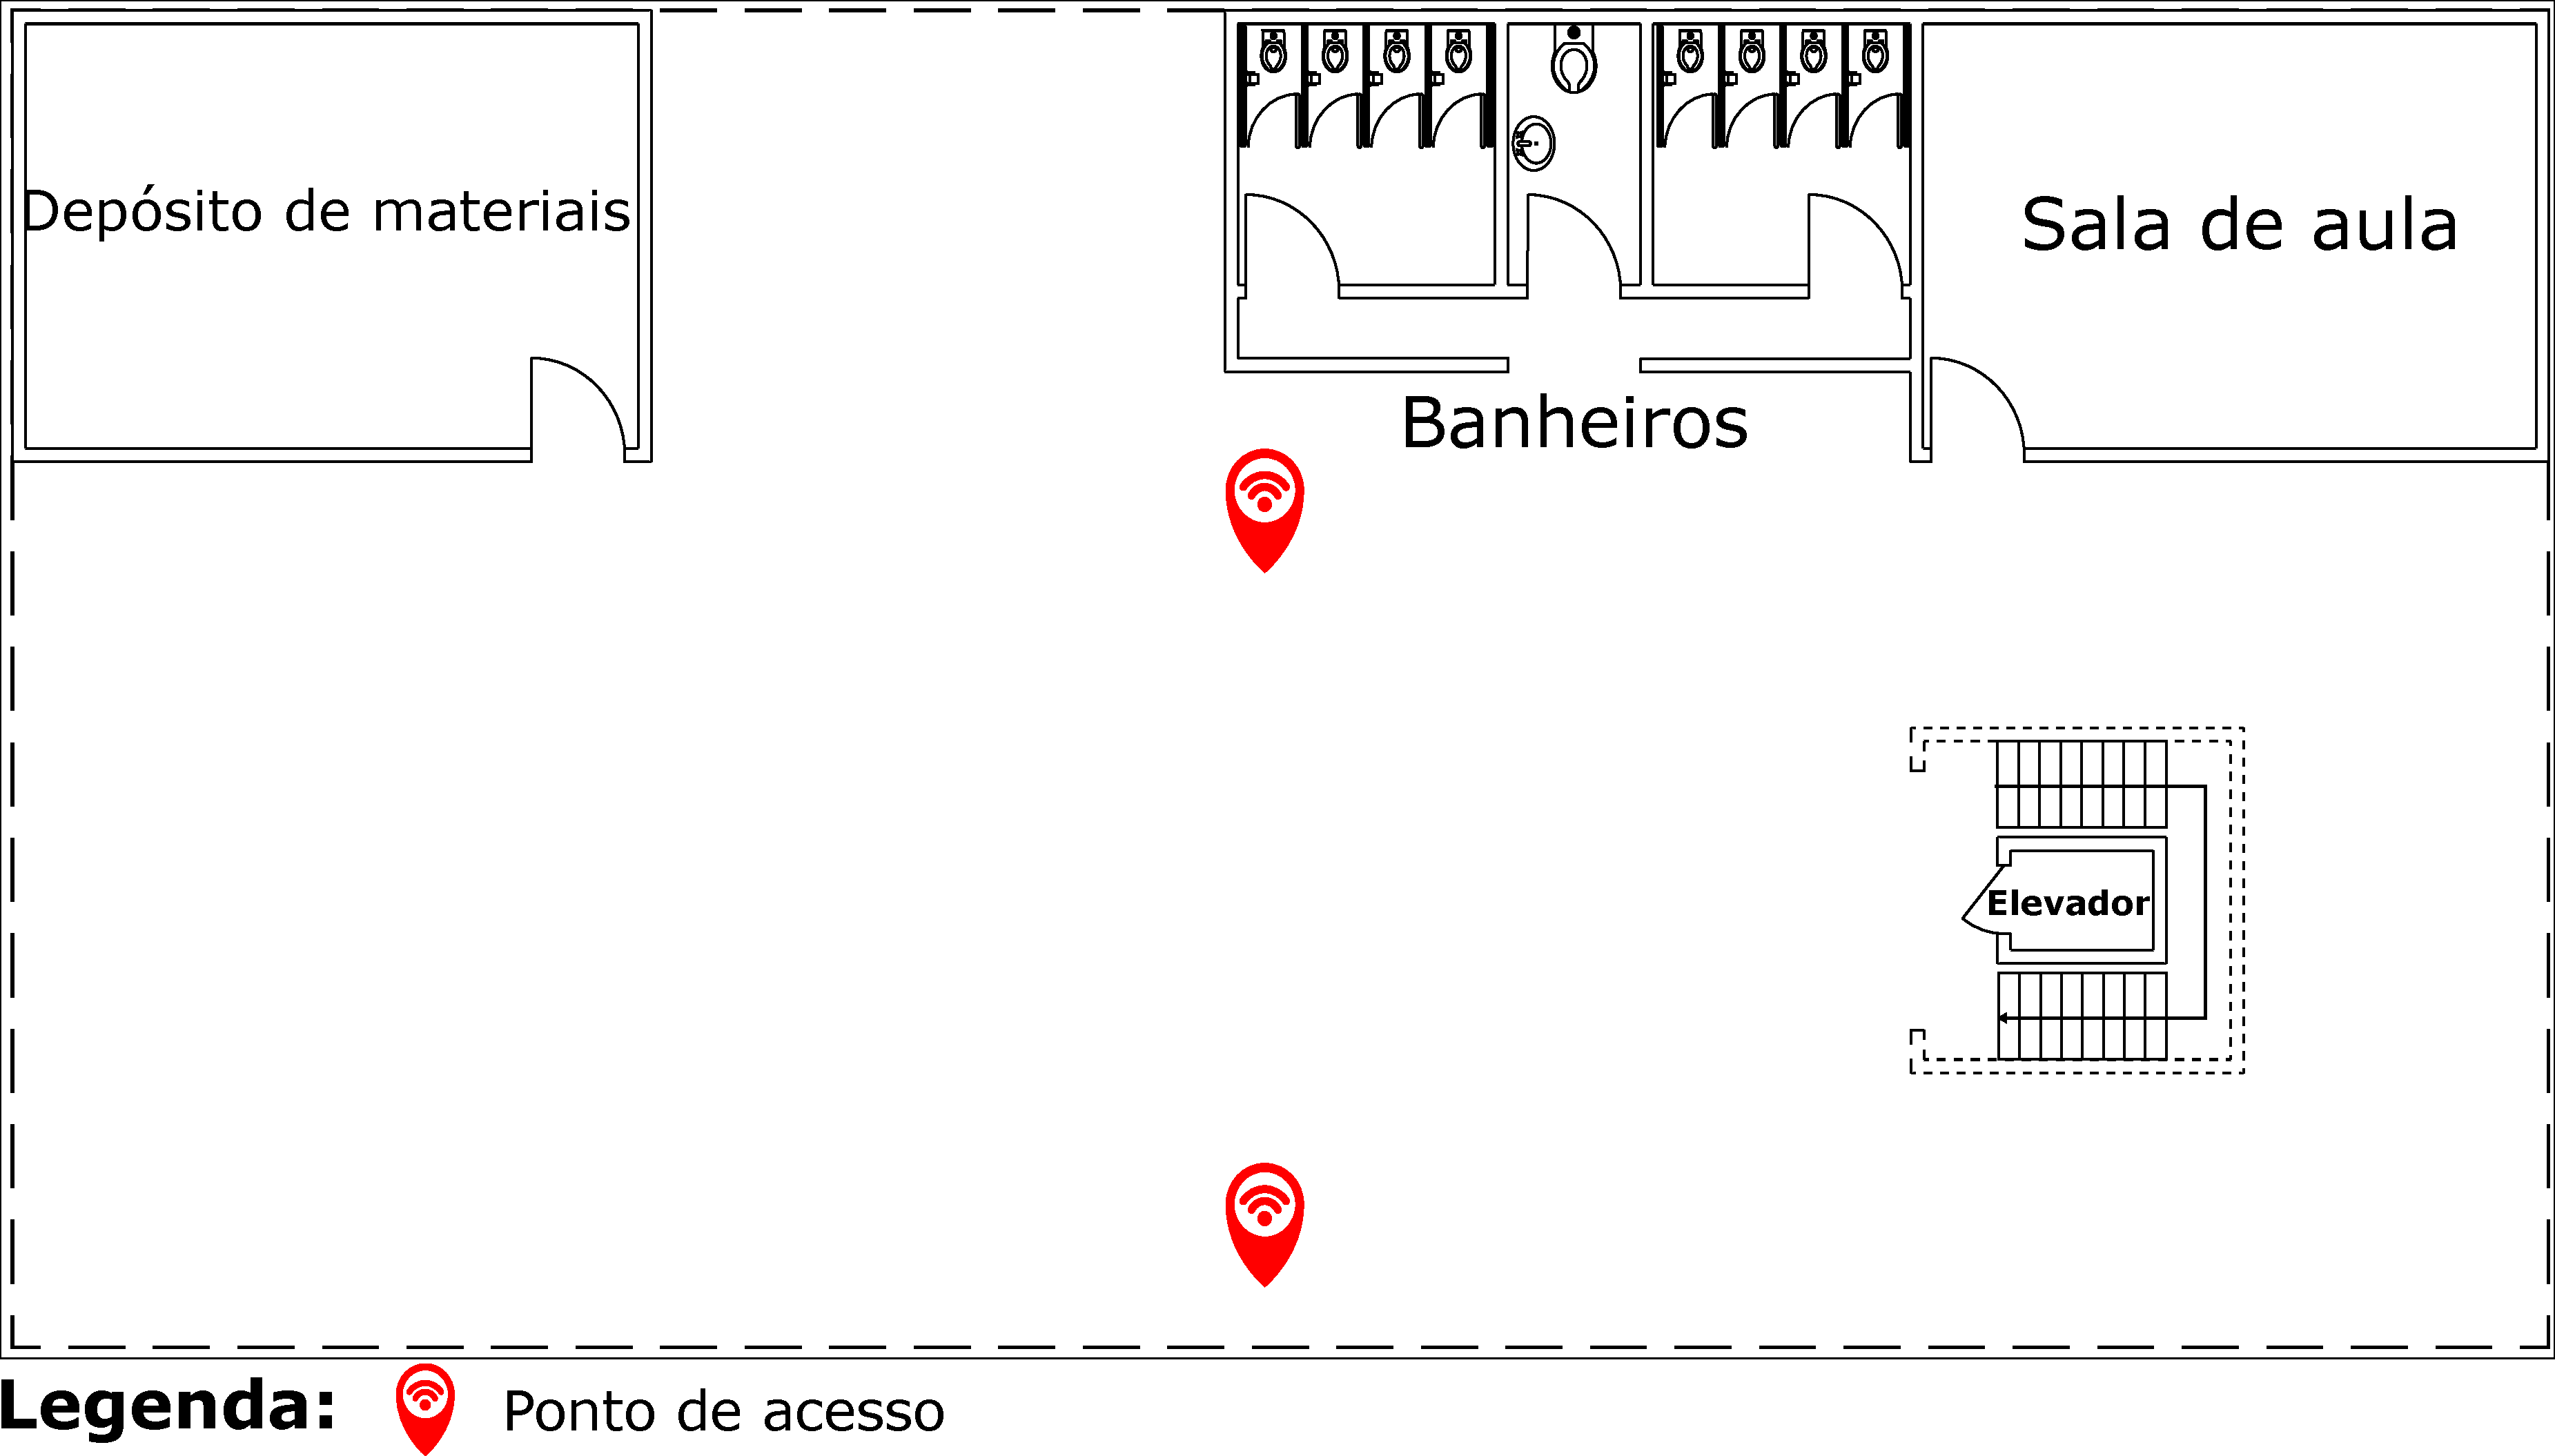
\includegraphics[scale=0.17]{fig_tcc/APs_Bloco_Andar_1_Proposta_Intervencao.pdf}
		\caption*{{\fontsize{8pt}{11}\selectfont Fonte: Autor.}}
	\end{figure}
\end{frame}
% ----------------------------------------- Slide -----------------------------------------
\begin{frame}{Proposta para Melhoria do Sinal}
	\framesubtitle{Segundo Andar}
	\begin{figure}[H]
		\centering
		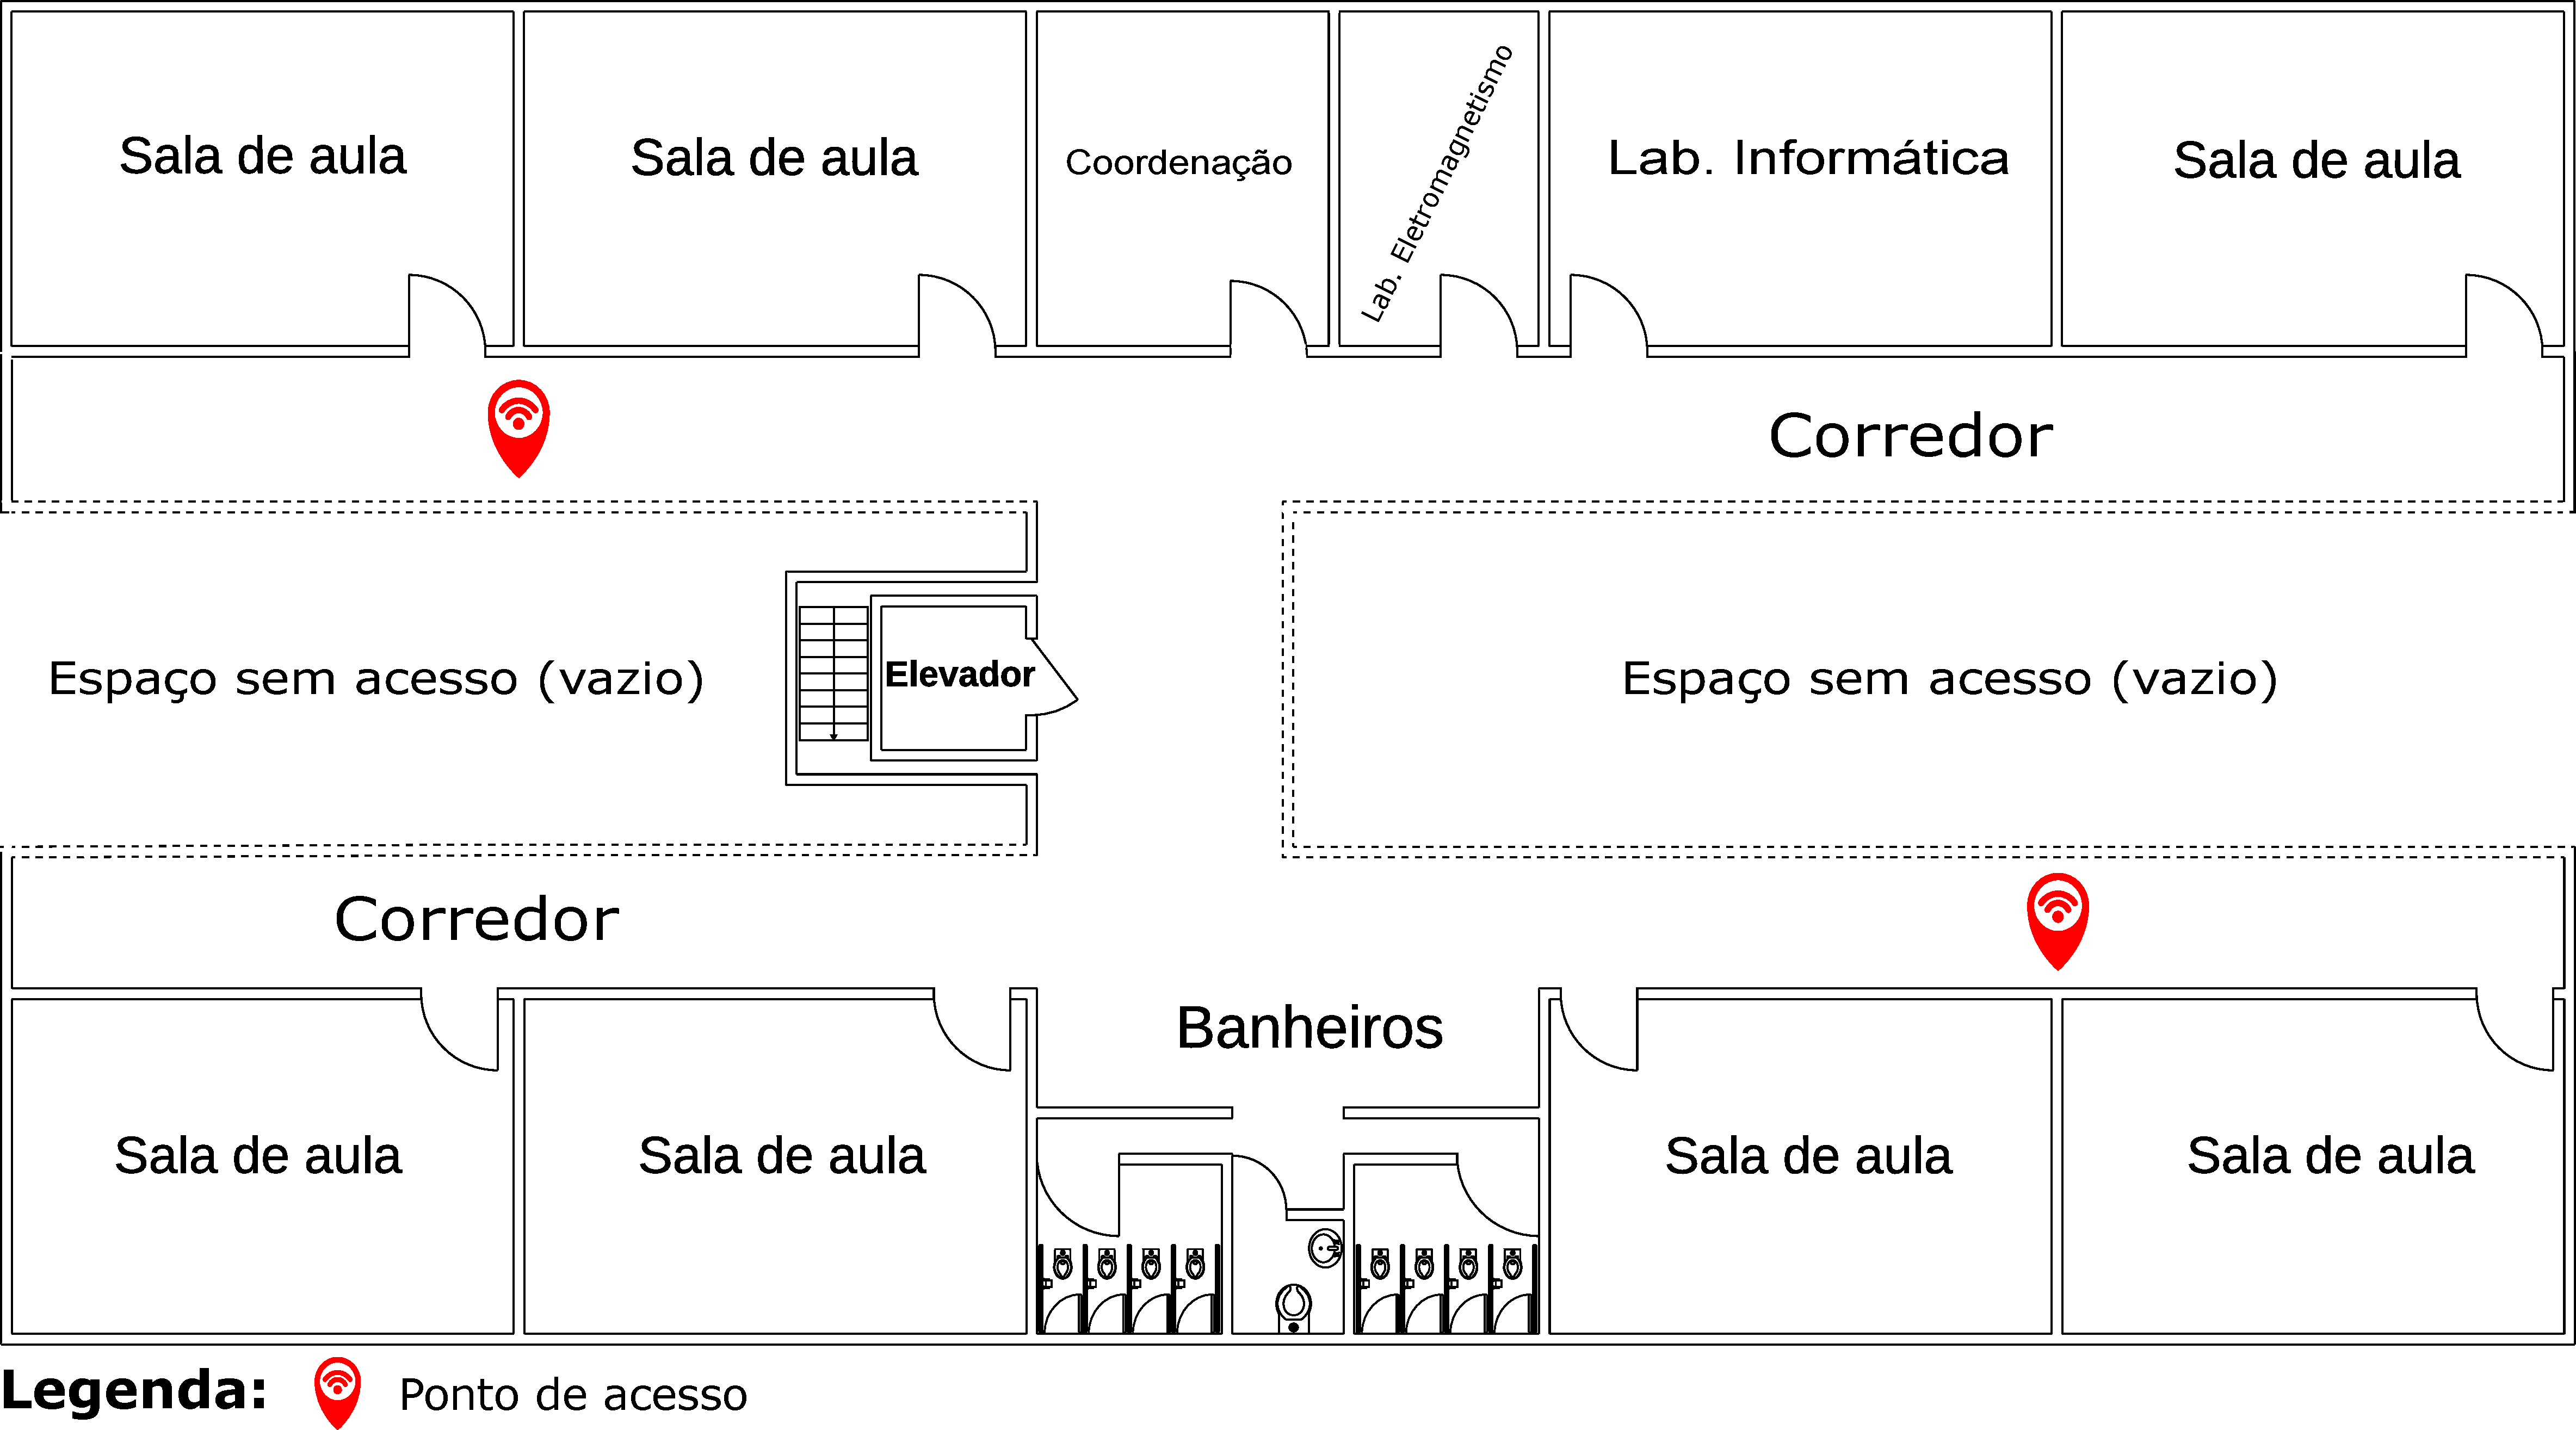
\includegraphics[scale=0.13]{fig_tcc/APs_Bloco_Andar_2_Proposta_Intervencao.pdf}
		\caption*{{\fontsize{8pt}{11}\selectfont Fonte: Autor.}}
	\end{figure}
\end{frame}
% ----------------------------------------- Slide -----------------------------------------
\section{Conclusão}
% ----------------------------------------- Slide -----------------------------------------
\begin{frame}{Considerações Finais}
	%\framesubtitle{Primeiro Andar}
	\begin{block}{}
		\begin{itemize}
			\item Canal de rádio impõe limitações no desempenho de sistemas de comunicações sem fio
				\begin{itemize}
					\item Caminho do sinal entre transmissor e receptor pode variar
				\end{itemize}
			\item Necessário a adoção de métodos de análise de redes \textit{wireless}
			\item \textit{Site survey} contribui para o ganho de desempenho de redes Wi-Fi
			\item Níveis de propagação de sinal diferentes para cada andar mapeado no trabalho
			\begin{itemize}
				\item Posicionamento dos pontos de acesso
				\item Andares com ambientes físicos distintos entre si
			\end{itemize}
		\end{itemize}
	\end{block}
\end{frame}
% ----------------------------------------- Slide -----------------------------------------
\begin{frame}[plain,c]
	%\framesubtitle{Primeiro Andar}
	\vfill
	\centering
	{\huge\textcolor{red}{\textbf{OBRIGADO PELA ATENÇÃO!!!}}}
	\vfill
\end{frame}
% ----------------------------------------- Slide -----------------------------------------
%\begin{frame}
%\frametitle{Referências}
%	\begin{thebibliography}{10}
%		\begin{scriptsize}
%		\justifying
%		\bibitem{beamer} CIRILO, Carlos E. \textbf{Computação Ubíqua:} definição, princípios e tecnologias. Artigo científico, Universidade Federal de São Carlos, São Paulo, 2008.
%		
%		\bibitem{beamer} COULOURIS, G.; DOLLIMORE, J.; KINDBERG, T. \textbf{Sistemas Distribuídos:} Conceitos e Projeto. 4. ed. Bookman Editora, 2007.
%		
%		\bibitem{beamer} DE ARAÚJO, Regina B. \textbf{Computação ubíqua:} Princípios, tecnologias e desafios. In: XXI Simpósio Brasileiro de Redes de Computadores, p. 11--13, 2003.
%		
%		\bibitem{beamer} NATÁRIO, Rui. \textbf{A Evolução da Computação:} A Era dos Mainframes. 2013. Disponível em: $<$\url{http://redes-e-servidores.blogspot.com/2013/02/a-evolucao-da-computacao-era-dos.html}$>$. Acesso em: 01 nov 2018.
%		
%		\bibitem{beamer} OTTOBBONI, João C. \textbf{Computação Ubíqua e Pervasiva.} 2014. Disponível em: $<$\url{https://pt.slideshare.net/jcottobboni/computao-ubqua-e-pervasiva}$>$. Acesso em: 01 nov 2018.
%		
%		\bibitem{beamer} SILVA, E.; BOTELHO, L.; SANTOS, I.; SANCHEZ, G. Computação Ubíqua -- Definição e Exemplos. \textbf{Revista de Empreendedorismo, Inovação e Tecnologia}, v. 2, n. 1, p. 23-32, 2015.
%		
%		\bibitem{beamer} WEISER, Mark. \textbf{The Computer for the 21 st Century}. In: Scientific american, v. 265, n. 3, p. 94--105, 1991.
%		\end{scriptsize}
%	\end{thebibliography}
%\end{frame}
% Fim da apresentação
\end{document}